\documentclass{article}

\usepackage{arxiv}

\usepackage{lipsum}

\usepackage[utf8]{inputenc} % allow utf-8 input
\usepackage[T1]{fontenc}    % use 8-bit T1 fonts
\usepackage{hyperref}       % hyperlinks
\usepackage{url}            % simple URL typesetting
\usepackage{booktabs}       % professional-quality tables
\usepackage{amsfonts}       % blackboard math symbols
\usepackage{nicefrac}       % compact symbols for 1/2, etc.
\usepackage{microtype}      % microtypography
\usepackage{graphicx}

\graphicspath{ {/} }

%\usepackage{natbib}
\usepackage{amsmath}
\usepackage{amssymb}
\usepackage{amsthm}
\usepackage{stmaryrd}
\usepackage{algorithmic,algorithm}
\usepackage{graphicx}
\usepackage{caption}
\usepackage{subcaption}
\usepackage{tikz}
\usepackage{dsfont}
\usetikzlibrary{positioning}
\usepackage{comment}

\makeatletter
\def\namedlabel#1#2{\begingroup
    #2%
    \def\@currentlabel{#2}%
    \phantomsection\label{#1}\endgroup
}
\makeatother


\newcommand{\cX}{\mathcal{X}}
\newcommand{\cL}{\mathcal{L}}
\newcommand{\cY}{\mathcal{Y}}

\newcommand{\bX}{\mathbf{X}}
\newcommand{\bY}{\mathbf{Y}}

% concatenation symbol (c.f. ++ in Haskell)
\newcommand\mdoubleplus{\mathbin{+\mkern-10mu+}}

% end of proof symbol
\newcommand{\newmarkedtheorem}[1]{%
  \newenvironment{#1}
    {\pushQED{\qed}\csname inner@#1\endcsname}
    {\popQED\csname endinner@#1\endcsname}%
  \newtheorem{inner@#1}%
}

\theoremstyle{definition}
%\newtheorem{eg}{Example}[section]
\newmarkedtheorem{eg}{Example}[section]
\newtheorem{observation}{Observation}[section]
\newtheorem{define}{Definition}[section]
\theoremstyle{plain}
\newtheorem{proposition}{Proposition}
\newtheorem{lemma}{Lemma}
\newtheorem{corollary}{Corollary}
\newtheorem{theorem}{Theorem}[section]
\newtheorem{assump}{Assumption}[section]
\newtheorem{remark}{Remark}[section]

\definecolor{fgcolor}{rgb}{0.345, 0.345, 0.345}
\newcommand{\hlnum}[1]{\textcolor[rgb]{0.686,0.059,0.569}{#1}}%
\newcommand{\hlstr}[1]{\textcolor[rgb]{0.192,0.494,0.8}{#1}}%
\newcommand{\hlcom}[1]{\textcolor[rgb]{0.678,0.584,0.686}{\textit{#1}}}%
\newcommand{\hlopt}[1]{\textcolor[rgb]{0,0,0}{#1}}%
\newcommand{\hlstd}[1]{\textcolor[rgb]{0.345,0.345,0.345}{#1}}%
\newcommand{\hlkwa}[1]{\textcolor[rgb]{0.161,0.373,0.58}{\textbf{#1}}}%
\newcommand{\hlkwb}[1]{\textcolor[rgb]{0.69,0.353,0.396}{#1}}%
\newcommand{\hlkwc}[1]{\textcolor[rgb]{0.333,0.667,0.333}{#1}}%
\newcommand{\hlkwd}[1]{\textcolor[rgb]{0.737,0.353,0.396}{\textbf{#1}}}%
\let\hlipl\hlkwb

\usepackage{framed}
\makeatletter
\newenvironment{kframe}{%
 \def\at@end@of@kframe{}%
 \ifinner\ifhmode%
  \def\at@end@of@kframe{\end{minipage}}%
  \begin{minipage}{\columnwidth}%
 \fi\fi%
 \def\FrameCommand##1{\hskip\@totalleftmargin \hskip-\fboxsep
 \colorbox{shadecolor}{##1}\hskip-\fboxsep
     % There is no \\@totalrightmargin, so:
     \hskip-\linewidth \hskip-\@totalleftmargin \hskip\columnwidth}%
 \MakeFramed {\advance\hsize-\width
   \@totalleftmargin\z@ \linewidth\hsize
   \@setminipage}}%
 {\par\unskip\endMakeFramed%
 \at@end@of@kframe}
\makeatother

\definecolor{shadecolor}{rgb}{.97, .97, .97}
\definecolor{messagecolor}{rgb}{0, 0, 0}
\definecolor{warningcolor}{rgb}{1, 0, 1}
\definecolor{errorcolor}{rgb}{1, 0, 0}
\newenvironment{knitrout}{}{} % an empty environment to be redefined in TeX



\title{Neural Combinatorial Optimization for Scalable Coordination of Autonomous
  Vehicles in Networks}

\author{
 Jeroen van Riel \\
Eindhoven University of Technology\\
  \texttt{j.a.a.v.riel@student.tue.nl} \\
}

\begin{document}
\maketitle

\begin{abstract}
  Autonomous vehicle coordination at intersections has the potential of reducing
  risk of accidents and providing significant savings in economic costs.
  %
  We propose to study coordination using an optimal control problem with hard
  collision-avoidance constraints to investigate the complexity of centralized
  traffic management without traffic signals.
  %
  With delay as the primary performance metric, we show how to decompose the
  high-dimensional formulation into two key components: (i) a variant of the
  classical job-shop scheduling problem and (ii) a trajectory optimization
  problem, which can be solved by linear programming.
  %
  Recent works have successfully applied reinforcement learning to derive
  scheduling policies for job-shop problems based on their disjunctive graph
  representation.
  %
  We propose to adapt this formalism to our variant and, building on previous
  works, to employ a graph neural network encoding of this extended disjunctive
  graph to parameterize a scheduling policy. The network can be trained using
  existing policy gradient algorithms, enabling the model to learn coordination
  stategies from scratch.
  %
  This approach offers an efficient approximation scheme, paving the way toward
  scalable solutions for more advanced coordination models.
\end{abstract}


\section{Overall aim and goals}

\subsection{Motivation and challenges}
\label{sec:motivation}

% context and overall motivation
Given the ongoing development of self-driving vehicle technology, it is not
difficult to imagine a future vehicular mobility system without human drivers.
Besides the obvious advantage of relieving us from the task of driving, freeing
time that can be spent on other activities, other benefits include
increased safety and efficiency. Human error is one of the major causes of most
accidents in vehicular traffic, which motivates the design of automated systems
with guarantees on collision avoidance, with the potential of saving millions of
injuries and lives. Furthermore, traffic coordination methods promise to reduce
economic costs such as travel delay, energy consumption and pollution~\cite{fagnantPreparingNationAutonomous2015}, by
optimizing the shared use of resources like parking lots and road intersections.
% scope
In general, coordination of autonomous vehicles has been studied at different
levels~\cite{marianiCoordinationAutonomousVehicles2022}. Local coordination like platooning of vehicles may lower energy
consumption by reducing aerodynamic resistance and may result in more efficient
use of intersections. On a larger scale, methods like network-wide dynamic route
optimization have been proposed to reduce travel delay for all users in the
traffic network.

We focus on coordination algorithms for optimizing the shared use of a network
of intersections without traffic lights. We consider a model in which each
vehicle in the network is managed by a central controller, illustrated in
Figure~\ref{fig:network_illustration}. Furthermore, we assume that every vehicle follows a
fixed predetermined route to explicitly ignore the problem of route generation.
%
In this context, we identify the following three key challenges
that are not yet fully addressed in the current literature.


\begin{itemize}

  \item \textbf{Safety.} It is nontrivial to design systems that are guaranteed
        to be safe with respect to collisions, because the potentially complex
        vehicle dynamics must be taken into account. Because safety is so
        crucial in real-world application, algorithms must guarantee this by
        design.

  \item \textbf{Scalability.} Most previous works consider coordination at a single
        intersection~\cite{khayatianSurveyIntersectionManagement2020} and involve algorithms that cannot be easily extended
        to multiple intersections. Coordination algorithms should naturally
        scale to complex real-world traffic networks with large numbers of
        vehicles. This requires a balance between the quality of solutions with
        computational complexity, motivating the study of good approximation
        schemes.

  \item \textbf{Learning.} Given the successful applications of (deep) reinforcement learning
        to a wide range of control tasks, it is natural to ask how
        coordination of autonomous vehicles can be formulated such that a
        similar methodology can be used to automatically learn good policies for
        this complex problem.
% constraint satisfaction
        The hard constraints, including collision avoidance, make it nontrivial to
        apply reinforcement learning in this case.
\end{itemize}

% recent neural JSSP success motivates further investigation
We observe that multi-intersection access control in a network of intersections
shows some resemblance to the classical job-shop scheduling problem, which is a
canonical example of a resource-sharing problem. For this type of problem, deep
reinforcement learning methods have recently been proposed~\cite{zhangLearningDispatchJob2020,zhangDeepReinforcementLearning2024}, often based on
efficient representations of problem instances using graph neural
networks~\cite{smitGraphNeuralNetworks2024}. This motivates us to investigate
whether a similar approach can be applied in our setting by adapting the
job-shop scheduling formulation to the autonomous traffic coordination problem.
Before we elaborate our proposed methodology, we briefly review existing works
and formulate concrete research questions to address the three identified
challenges.


\subsection{Overview of related literature}

Traffic lights are currently one of the most effective way of guiding traffic,
so current coordination methods often rely on some sort of synchronization of
traffic light settings at neighboring intersections~\cite{mcshaneTrafficEngineering1990,hePAMSCODPlatoonbasedArterial2012}, with \textit{green waves} on
arterial roads being a well-known example. Since the complex interactions in
signalized networks are difficult to model using basic principles, recent years
have seen an increased interest in the application of deep learning models to
traffic-related problems. In particular, numerous works have successfully
proposed deep reinforcement learning methods for traffic signal control that
scale to large networks of intersections~\cite{noaeenReinforcementLearningUrban2022,weiSurveyTrafficSignal2020}.
%
Most of these works involve human-driven vehicles and rely heavily on precise
models of the corresponding vehicle dynamics using so-called microscopic
simulators~\cite{lopezMicroscopicTrafficSimulation2018}.

Given the increasing number of fully autonomous vehicles, new types of traffic
coordination schemes have become conceivable~\cite{marianiCoordinationAutonomousVehicles2022}, with notable examples being
services like smart parking and ride-sharing, local coordination methods like
ramp merging and platooning, or network-wide traffic flow optimization through
smart route suggestions.
%
Intersection access management without traffic signals is one type of setting in
which coordination of autonomous vehicles can potentially bring huge benefits,
both in terms of reduced risk and economic costs. While early works were mostly
based on reservation-based protocols~\cite{dresnerMultiagentApproachAutonomous2008}, current coordination schemes are
studied under a wide range of model assumptions regarding vehicle dynamics and
modes of communication and control~\cite{khayatianSurveyIntersectionManagement2020}. An important distinction can be made
based on the used communication models, which can be roughly categorized into
distributed approaches, where groups of vehicles coordinate trajectories
together, and centralized approaches, where individual vehicles receive
instructions from a central controller.

\begin{figure}[b]
  \centering
  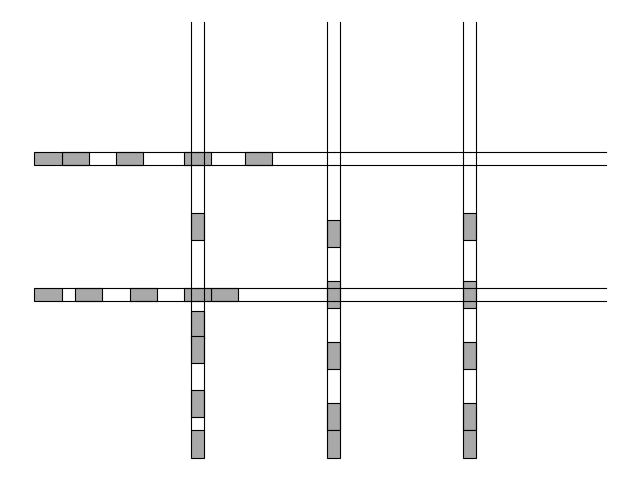
\includegraphics[width=0.5\textwidth]{figures/state_example.png}
  \caption{Illustration of some simple grid-like network of intersections
    with vehicles drawn as grey rectangles. There are five vehicle routes that
    only intersect at intersections (so no two routes share the same lane
    between intersections): two from east to west and three from south to north.
    Turning at intersections is not allowed in this
    model.}\label{fig:network_illustration}
\end{figure}

Centralized approaches mostly ignore issues with communication and distributed
computing in order to study intersection access management under the optimal
control framework, providing a sound theoretical foundation. Most works from
this perspective use a simple one-dimensional vehicle model known as the double
integrator in optimal control literature~\cite{raoNaiveControlDouble2001}. In
principle, solutions can often be obtained using so-called \textit{direct transcription}
methods, but the high-dimensionality of the problem calls for good approximation
schemes to keep computational expenses balanced. A common observation is that
the problem may be thought of as two coupled optimization problems~\cite{hultApproximateSolutionOptimal2015,zhaoBilevelProgrammingModel2021,tallapragadaHierarchicaldistributedOptimizedCoordination2017}, where
the upper-level problem is to determine when and in which order vehicles enter
and exit each intersection on their route. The lower-level problem is to find
optimal trajectories that match these time slots.

Extensions to multi-intersection access management have received much less
attention. Existing methods are extensions of reservation-based protocols~\cite{hausknechtAutonomousIntersectionManagement} or
are based on mixed-integer linear programming~\cite{sartorCombinatorialLearningTraffic2019}.
% neural combinatorial optimization
As the remainder of this proposal will show, we recognize that the additional
complexity of the multi-intersection extension is in large part of a
combinatorial nature. At the same time, we observe that recent literature shows
an increasing interest in applying a machine learning perspective on
combinatorial problems~\cite{bengioMachineLearningCombinatorial2020,lodiLearningBranchingSurvey2017}, to which we refer as \textit{neural combinatorial
  optimization}. Realistic instances of many combinatorial
problems are often too complex to solve to optimality, so researchers try to
propose good approximation schemes and heuristics, based on some kind of
structure in the problems of interest. However, manually designing such
heuristics is a tedious task, requiring a lot of experience and deep insight
into the problem. Recently, tailored deep reinforcement learning methods have
shown to be able to automatically derive good heuristics from scratch for many
classical combinatorial optimization problems~\cite{belloNeuralCombinatorialOptimization2017,koolLearningOptimizationCombinatorial,mazyavkinaReinforcementLearningCombinatorial2020,smitGraphNeuralNetworks2024}.


\subsection{Problem formulation and research questions}

% problem formulation
We study a centralized model for the network-wide coordination of autonomous
vehicles, in which vehicles are directly controlled without relying on traffic
lights. Specifically, we model coordination as an optimal control problem with
hard constraints on collision avoidance and assume a perfect
communication and control setup. The central controller determines the
acceleration of each vehicle, modeled as a rectangle that moves according to double
integrator dynamics. Once a vehicle enters the network, it follows a predetermined route
until it exits, as illustrated in Figure~\ref{fig:network_illustration}. The
goal is to control the trajectory of each vehicle in the network, ensuring
collision-free movement while optimizing a global measure of efficiency. One
common measure of efficiency in the literature is the total delay experienced by
all vehicles. However, it may also be desirable to penalize acceleration, which
can serve as a proxy for energy consumption. In scenarios where all vehicle
arrival times are known in advance, we assume that the trajectories can be
computed offline, without any prior interaction with the system. This problem setup is
referred to as \textit{offline trajectory optimization}.

In general, the offline trajectory optimization problem is of infinite
dimension, because vehicle trajectories are smooth functions of time. Therefore,
every numerical algorithm must introduce some kind of dimensionality reduction
scheme. In this case, we recognize some basic structure that allows us to define
a lower-dimensional problem formulation.
%
By assuming that the vehicle dynamics are known precisely, it is possible to
formulate hard constraints on the trajectories of vehicles in order to avoid
collisions. One key observation is that these constraints are somewhat similar
to those found in classical job-shop scheduling problems, where vehicles and
intersections correspond to jobs and machines, respectively. Efficient solution
methods are available for this type of problem, scaling reasonably well to
larger instances.
%
Therefore, we aim to address the first two challenges of safety and scalability
by answering our first research question:
%
\begin{enumerate}
  \item[\textbf{\namedlabel{Q1}{Q1}}.] How can we model the offline trajectory optimization
        problem, modeling coordination of autonomous vehicles in networks of
        unsignalized intersections, as a variant of job-shop scheduling to
        effectively reduce the dimensionality of the problem, while guaranteeing
        the generation of collision-free trajectories?
\end{enumerate}

Apart from the similarity to job-shop scheduling, we believe that the offline
trajectory optimization problem has additional structure related to the way in
which vehicle trajectories interact in large networks of intersections. Our
second aim is to investigate how deep reinforcement learning can be applied to
the offline trajectory optimization problem, because we believe that a machine
learning perspective~\cite{bengioMachineLearningCombinatorial2020} can help model hidden regularities in complex
decision-making problems. Our hypothesis is that it is generally hard to
manually design algorithms that exploit such structural features, so
reinforcement learning might be employed to automatically learn to do this based
on interaction with problem instances. Therefore, to further improve the scalability of
our solutions method and to address the remaining challenge of learning, we
formulate our second research question as:
%
\begin{enumerate}
  \item[\textbf{\namedlabel{Q2}{Q2}}.] Can recent deep reinforcement learning formulations for
        combinatorial optimization problems, like job-shop scheduling, be
        adapted to the offline trajectory optimization problem, formulated in
        terms of job-shop scheduling, in order to provide a scalable
        optimization algorithm that automatically learns to exploit hidden
        structures in problem instances?
\end{enumerate}


\newpage

\section{Research approach}

\subsection{Overall methodology and decomposition}

% infinite dimensional -> direct transcription
Because trajectories are smooth functions, the offline trajectory optimization
problem is generally of infinite dimension. In order to solve it numerically,
some dimensionality reduction scheme is required. A straightforward way to
represent trajectories is based on a discrete time grid. Based on this, it is
possible to formulate a mixed-integer linear program, whose optimal solutions
approximate solutions to the original problem. Such so-called \textit{direct
  transcription} methods are very common for optimal control problems, but they
are still very high-dimensional due to the time discretization.

% bilevel decomposition
We show how the dimension can be reduced further, based on the following
observation. A key issue the controller has to decide is the order of crossing
at intersections, which is precisely what makes the optimal control problem
non-convex and thus hard to solve with standard methods. When considering an
optimization objective in terms of vehicle delay and some additional
assumptions, the problem can be shown to decompose as a \textit{bilevel} optimization
problem with an \textit{upper-level} combinatorial problem to determine a crossing time
schedule --- indicating when vehicles cross the intersections on their route
--- and a \textit{lower-level} optimal control problem to find trajectories that match
these crossing times, see Figure~\ref{fig:network_bilevel} for an illustration.

\begin{figure}[h]
  \centering
  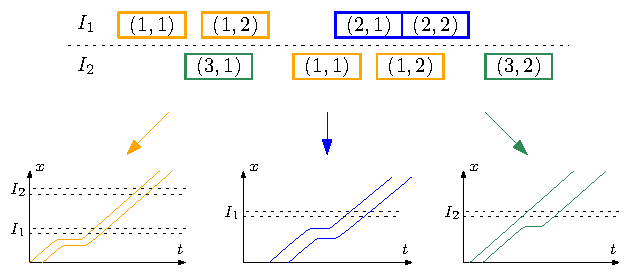
\includegraphics[width=0.8\textwidth]{figures/network_bilevel.pdf}
  \caption{Illustration of the proposed bilevel decomposition. The upper-level
    problem is assign each vehicle a time slot for each of the intersections
    (here denoted $I_{1}$ and $I_{2}$) on its route. Based on this schedule, the
    lower-level problem is to generate trajectories satisfying these time
    slots.}
  \label{fig:network_bilevel}
\end{figure}

% upper-level: job shop scheduling variant
Under some assumptions on the routes that vehicles take, it can be shown that
the upper-level problem, to which we will refer as the Vehicle Scheduling
Problem (VSP), is an extension of the classical Job-Shop Scheduling Problem
(JSSP). Intersections are modeled as machines (the shared resources) and each
vehicle corresponds to a job, whose operations model the crossing of
intersections on the vehicle's route.
%
In addition to the regular JSSP constraints, three types of additional
constraints are defined to model some necessary clearance time at intersections
and to take into account the travel time between intersections and safety
constraints to prevent rear-end collisions.
% lower-level efficient
Given a solution to the VSP, computing the lower-level trajectories can be done
reasonably efficiently, as we show in the next section. Furthermore, it can be
shown that trajectories that satisfy the schedule are guaranteed to
be collision-free, satisfying our first objective of guaranteed safety.
% focus on upper-problem
Therefore, the bilevel decomposition enables us to focus on solving the
scheduling problem.

% 1. MILP
Like plain JSSP problems, VSP can be solved by formulating it as a Mixed-Integer
Linear Program (MILP) and using an off-the-shelf solver. Although being a
powerful optimization framework, this approach is not likely to scale well,
because of the inherent complexity of larger instances. However, by setting a
time limit on the solving time, this method yields a good heuristic solution
method.

% 2. neural COP
To tackle the scalability issue, we propose to leverage the recent progress made
in applying Deep Reinforcement Learning (DRL) methods to Combinatorial
Optimization Problems (COP), of which JSSP is a classical example. We show that
the disjunctive graph encoding of job-shop problems can be extended to our VSP
variant. Following the approach of previous successful deep reinforcement
learning methods for job-shop problems, we propose a policy for generating
schedules in a step-by-step fashion. The policy is parameterized based on a
Graph Neural Network (GNN) encoding of the adapted disjunctive graph. We verify
whether the resulting policy space is general enough by using imitation learning
on expert demonstration obtained from optimal solutions by backtracking the
required step-by-step decisions. Finally, we train the policy using
reinforcement learning in a step-by-step scheduling environment.


\subsection{Models and methods}

We now provide a more detailed introduction of the most important models and
methods that we plan to use and discuss how they can be adapted to the current
problem formulation. The first three sections are mainly about answering
research question~\ref{Q1} by defining the upper-level Vehicle Scheduling
Problem. Section~\ref{sec:constructive_neural} shows how to solve this problem
using deep reinforcement learning, thereby answering question~\ref{Q2}.

\subsubsection{Trajectory optimization}

% vehicle dynamics and feasibility
The bilevel decomposition sketched above depends heavily on the feasibility of
the lower-level trajectory optimization problem. More precisely, we need to be
sure that a crossing time schedule always allows trajectories that respect the
vehicle dynamics and are collision-free.
% three different crossing snapshots
Therefore, we distinguish three key moments in time related to a particular
crossing. For some combination of an intersection and a vehicle with this
intersection on its route, let the \textit{crossing time} $y$ be the first
moment when the front bumper of the vehicle $i$ enters the intersection area, as
depicted by the first situation in Figure~\ref{fig:vehicle_crossing}. Next, let
$\rho > 0$ denote the time after which another vehicle on the same route can
start crossing and let $\sigma > \rho$ denote the duration of a \textit{full crossing},
after which any vehicle from a conflicting route can start
crossing the intersection.
% assumption on v=vmax on whole crossing time slot
To simplify matters, we assume that vehicles drive at \textit{full speed} when crossing
the intersection, so for all $t$ between $y$ and $y + \sigma$.

\begin{figure}[h]
  \centering
  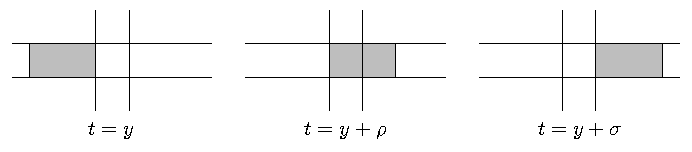
\includegraphics[width=0.7\textwidth]{figures/vehicle_crossing.pdf}
  \caption{Three different snapshots of a vehicle crossing an intersection.}
  \label{fig:vehicle_crossing}
\end{figure}

% separate optimal control problems per route
The upper-level scheduling problem provides the crossing times $y$,
which the trajectories must satisfy. Together with the constraints from the
double integrator vehicle dynamics, this yields a separate optimal control
problem for each group of vehicles with the same route.
% direct transcription
Each of these can be straightforwardly solved by direction transcription to a
linear program by introducing a discrete time grid to represent each vehicle's
trajectory. The vehicle dynamics can be encoded using a forward Euler scheme or
higher-order numerical integration methods. Rear-end collision-avoidance
constraints can simply be added for each time step. Finally, the position at
time step $y$ is bound to the start of the intersection.


\subsubsection{Job-shop scheduling}

We briefly introduce the Job-Shop Scheduling Problem (JSSP), because we
formulate our Vehicle Scheduling Problem (VSP) as a direct extension. For a
textbook introduction, we recommend the very accessible book on scheduling by
Pinedo~\cite{pinedoSchedulingTheoryAlgorithms2016}.
%
The classical JSSP problem considers a set of $n$ jobs that must be assigned to
non-overlapping time slots on a set of $m$ machines. Each job $i$ has a set of
$n_{i}$ operations $O_{i1}, \dots, O_{in_{i}}$ that need to be executed in this
order. Each operation $O_{ij}$ requires $p_{ij}$ processing time on machine
$M_{ij}$. Each machine can process at most one operation and early preemption is
not allowed. The task of the scheduler is to determine a valid schedule of start
times $y_{ij}$ for each operation, while minimizing some objective function. Let
$C_{ij} = y_{ij} + p_{ij}$ denote the \textit{completion time} of operation $O_{ij}$.
Common optimization objectives are a function of these completion times, e.g.,
minimizing the total completion time among operations or minimizing the maximum
completion time, also known as the \textit{makespan}. Objectives that are a
non-decreasing function of completion times are called \textit{regular}.

% disjunctive graph
A commonly used representation of JSSP instances is the \textit{disjunctive
  graph}, with vertices $\{ O_{ik} : 1 \leq i \leq n, 1 \leq k \leq n_{i} \}$
corresponding to all the operations. The set of \textit{conjunctive arcs} encodes
all the precedence constraints $O_{i,k} \rightarrow O_{i,k+1} $ among each job's
operations. The set of \textit{disjunctive edges} consists of undirected edges
between each pair of operations from distinct jobs that need to be processed on
the same machine, effectively encoding all such \textit{conflicts}. Each valid
schedule induces an ordering of operations on machines that is encoded by fixing
the direction of each disjunctive edge such that we obtain a directed acyclic
graph.

\begin{figure}[h]
  \centering
  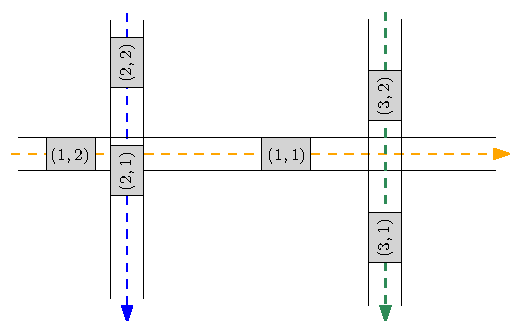
\includegraphics[width=0.65\textwidth]{figures/network_indices.pdf}
  \caption{Example network with three different routes satisfying the
    edge-disjoint assumption (such that vehicle flows never merge) and vehicle
    indices $(r,k)$.}
  \label{fig:network_indices}
\end{figure}

We now explain how JSSP can be extended to VSP, where intersection are modeled
as machines, vehicles correspond to jobs.
% network graph, crossing <-> operation
The road network is represented as a simple directed graph with nodes
representing intersections. Each vehicle has a fixed route consisting of a
series of intersections. The act of \textit{crossing} an intersection on this
route is modeled as an operation. The processing time of a crossing corresponds
to $\rho$ in Figure~\ref{fig:vehicle_crossing}.
% edge-disjoint routes, no overtaking => (r,k) indices
We assume that routes are \textit{edge-disjoint}, in the sense that they do not
share edges but possibly overlap at nodes (intersections). Furthermore, we
assume that vehicles on the same lane are not able to overtake. Therefore, each
vehicle can be identified as a tuple $(r, k)$, with some route identifier $r$
and an integer $k$ that indicates the relative order on this route, see
Figure~\ref{fig:network_indices} for an example. In addition to the regular
constraints of JSSP, we define the following three constraints:

\begin{itemize}
  \item \textit{Clearance time.} To guarantee collision-free crossing at
        intersections, some additional time is required between crossing times
        for vehicles that approach an intersection from different lanes. More
        precisely, we require at least $\sigma$ time (see
        Figure~\ref{fig:vehicle_crossing}) between crossings of vehicles
        belonging to different routes.

  \item \textit{Travel constraints.} Vehicles need to physically drive towards
        the next intersection on their route, so there is a lower bound on
        the travel time. Therefore, we need a constraint between the crossing
        times at every two consecutive intersections on each vehicle's route.

  \item \textit{Buffer constraints.} Each lane between intersections has only
        space for a limited number of vehicles, depending on their position and
        velocity. To avoid rear-end collisions, the number of vehicles in each
        lane needs to be limited.
        %
        This type of constraint is the most difficult to formulate, so the basic
        principle is illustrated by the example in
        Figure~\ref{fig:buffer_constraints}.
\end{itemize}

\begin{figure}[h]
  \centering
  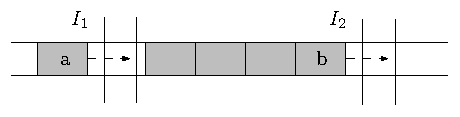
\includegraphics[width=0.55\textwidth]{figures/buffer_constraints.pdf}
  \caption{Illustration of buffer constraint for a pair of vehicles on the same
    route. Suppose that the vehicles on the lane between the two intersections
    are currently not moving and waiting to cross $I_{2}$. It is clear that the
    crossing time of vehicle $a$ at $I_{1}$ must happen at least after
    vehicle $b$ starts crossing $I_{2}$. Since this particular lane segment has
    capacity for 4 waiting vehicles, we need such a buffer constraint between
    every pair of vehicles $(r,k_{1})$ and $(r,k_{2})$ that satisfy
    $k_{2} = k_{1} + 3$.}
  \label{fig:buffer_constraints}
  \end{figure}

%{\color{blue} discuss simple heuristics (based on priority rules)}

\subsubsection{Mixed-integer linear programming}

% mixed-integer programming
Like the original JSSP, our VSP can be formulated as a Mixed-Integer Linear
Program (MILP).
% single intersection
For a single isolated intersection, it is straightforward to do this. The
crossing order decisions can be modeled by introducing a binary decision
variable for each pair of conflicting vehicles that approach the intersection
from different lanes. Note that the number of these so-called
\textit{disjunctive decisions} grows exponentially in the number of vehicles.
% platoon preservation
Whenever two consecutive vehicles on the same lane are able to cross the
intersection without a gap, it has been shown that they will always do so in any
optimal schedule~\cite{limpensOnlinePlatoonForming2023} (with respect to the
total delay objective).

% network: addresses scalability objective
When considering a network of intersections, the two additional types of constraints
are necessary to guarantee feasibility of the lower-level trajectory
optimization.
% both constraints can be encoded in disjunctive graph
Both constraint types can be naturally encoded in the disjunctive graph.
%
When we assume that there is no merging of routes, which means they only overlap
at intersections, we expect that VSP is still computationally tractable for
reasonably sized instances, using modern solvers. Whenever general routes
are considered, a naive formulation would include a lot of disjunctive
decisions, because vehicles can in principle conflict with all other vehicles
that share a part of their route, even if it is clear that this would never
happen in any sensible schedule.

During the solving procedure, the current best solution is remembered.
Therefore, MILP solving can be used as an approximation method by setting a
limit on the computation time, which addresses our second overall objective.
%
Another benefit of the MILP framework is the easy incorporation of
problem-specific \textit{cutting planes} in order to exploit additional
structure in problem instances. For example, we observe that the above property
on crossing without a gap in a single intersection can be used to formulate
multiple types of cutting planes to improve the running time of the solver.


\subsubsection{Constructive neural heuristic}
\label{sec:constructive_neural}


% neural combinatorial optimization
We now explain how to model VSP as a sequential decision making process such
that deep reinforcement learning can be applied to address our objective of
obtaining a learning optimization algorithm.
% determine crossing order
The fundamental challenge of the scheduler is to determine in which order
vehicles are allowed to cross the intersections on their routes. Observe that
the relative order among vehicles on the same route stays fixed, because they
are not allowed to overtake.
%
We propose to order vehicles in a step-by-step fashion. For each intersection,
we keep track of a partial ordering of vehicles. Each step corresponds to
choosing some combination of an intersection and a vehicle that has not yet been
added to the partial ordering of this intersection and has this intersection on
its route. We will refer to such intersection-vehicle pair as a \textit{crossing}.
Figure~\ref{fig:network_ordering} illustrates an example of a partial ordering after four steps.

\begin{figure}[h]
  \centering
  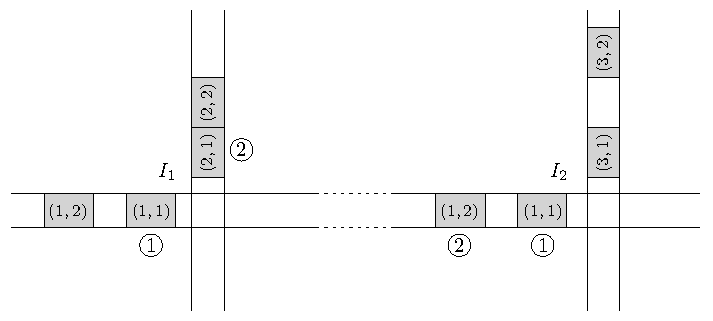
\includegraphics[width=0.9\textwidth]{figures/network_ordering.pdf}
  \caption{Illustration of some partial ordering, indicated by the encircled
    numbers. The order among vehicles without an encircled number is still to be
    decided by the scheduler, bust must respect the fact that vehicles on the
    same route cannot overtake. In this particular example, this means that the
    crossing order at $I_{2}$ can only be completed in one way.}
  \label{fig:network_ordering}
\end{figure}

This step-by-step process can be cast into the Markov Decision Process (MDP)
framework.
% state is partial ordering and action is (intersection, vehicle) pair
The state corresponds to the current partial ordering and each action
corresponds to a valid intersection-vehicle pair to add to the partial ordering.
Observe that the MDP is completely deterministic by definition. As we will show
next, a complete ordering of vehicles induces a complete schedule with exact
crossing time slots, so we may simply define an episodic reward in terms of the
total delay of the final schedule.
% disjunctive graph to encode partial ordering
The disjunctive graph, see Figure~\ref{fig:disjunctive_graph}, provides a way to
encode a partial ordering by specifying the direction of a selection of
disjunctive edges.
% lower bounds in partial disjunctive graph
Using the resulting \textit{partial disjunctive graph} we can derive lower bounds on the crossing
times. Recall that every node of the disjunctive graph corresponds to a crossing
and that every arc corresponds to some constraint. We can derive lower bounds on
the crossing times based on all the constraints whose arc has been added to the
partial disjunctive graph by solving a linear program.
% efficient LB update
However, we think that it is possible to develop a tailored update scheme that
only propagates the necessary changes over the partial disjunctive graph
whenever a set of disjunctive arcs is added.
% complete ordering => complete schedule
Finally, it is not difficult to see that the lower bounds for a complete ordering are
precisely the crossing times of the corresponding schedule.

\begin{figure}[h]
  \centering
  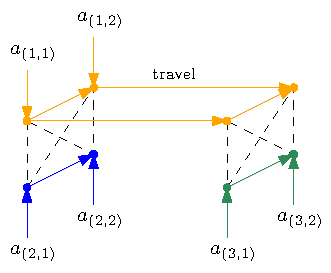
\includegraphics[width=0.5\textwidth]{figures/disjunctive_graph.pdf}
  \caption{Illustration of a disjunctive graph corresponding to the instance in
    Figure~\ref{fig:network_bilevel} with respect to the network from
    Figure~\ref{fig:network_indices}. For each route, conjunctive arcs are drawn
    at a slight angle and the horizontal arcs correspond to the travel
    constraints (only applicable to vehicles on route 1). The dashed lines
    represent disjunctive edges for the two intersections. For each node
    corresponding to the first intersection on the route $r$, an incoming arc
    labeled $a_{(r,k)}$ represents the earliest arrival time constraints. Buffer
    constraints are not shown, as they are not applicable to this small
    example.}
  \label{fig:disjunctive_graph}
\end{figure}

We will now discuss how to parameterize the scheduling policy, which is a
function from a partial solution (partial disjunctive graph) to an action
(crossing).
% disjunctive graph -> GNN -> encoding of partial solution
Previous works have been able to train good policies based on encodings of the
disjunctive graph for JSSP. Following this direction, we propose build
an encoding of the partial disjunctive graph augmented with the corresponding
crossing time lower bounds.
%
Graph Neural Networks (GNN) are deep neural networks that are suited to encode
graph-structured data from node-level features. For each node in the (partial)
disjunctive graph, we record two basic features: (i) a binary variable
indicating whether this crossing has already been scheduled and (ii) the current
crossing time lower bound. By iteratively combining these node-level features in
a parameterized non-linear fashion, we obtain an embedding $h_{O}$ for every
node $O$ and a global graph embedding $O_{\mathcal{G}}$. These embeddings are
then mapped to an action distribution via a fully connected net and softmax
function.
% size-agnostic
As already noted in~\cite{zhangLearningDispatchJob2020}, such an architecture has the major advantage of being
size-agnostic, meaning that the same policy can be applied to other instances
with a different network and varying number of vehicles.

% imitation learning
We will consider two learning paradigms for tuning the parameters in order to
obtain good policies. In the \textit{imitation learning} setting, the policy is
trained to imitate expert demonstration. For example, we can use a MILP solver
to obtain the optimal schedule and then backtrack the corresponding state-action
pairs that our policy must take in order to arrive at the same schedule. These
resulting training set of state-action pairs can then be used to tune the policy
in order to mimic the expert policy as closely as possible.
% reinforcement learning
When expert demonstration is not available, we can directly learn from
interaction with the MDP, which is what is generally known as \textit{reinforcement
  learning}. Policy parameters are tuned using a policy gradient
learning algorithm like the classical REINFORCE~\cite{10.1007/BF00992696} or the
more recent Proximal Policy Optimization
\cite{schulmanProximalPolicyOptimization2017}.


\subsection{Research plan and timeline}


Time estimates are based on a total duration of 30 weeks (three quartiles of 10
weeks each) of which the last four weeks are reserved for report writing and
preparing material for a final presentation.

\begin{itemize}
  \item (done) \textbf{Direct transcription of lower-level.} The proposed bilevel
        decomposition depends heavily on our ability to solve the lower-level
        problem efficiently. Therefore, our first effort should be to develop a
        working direct transcription solution to obtain trajectories for a given
        crossing time schedule.

  \item (2 weeks) \textbf{Upper-level formulation.} We precisely formulate VSP for
        networks with delay objective (network scheduling problem).
        Particularly, this mainly involves formulating the travel constraints
        and buffer constraints such that feasibility of the lower-level problem
        is guaranteed. At this stage, we only aim to provide a rough proof
        sketch of this, because we simply verify this feasibility

        %{\color{blue} We are almost done with this, the only missing part is a clear argument
        %of why we expect our current version of buffer constraints to work.}

  \item (1 week) \textbf{MILP for VSP.} Solve the network scheduling problem by formulating and
        solving it as a MILP. This method can be used to collect expert
        demonstrations for training the neural scheduler using imitation
        learning and it also provides a baseline for performance evaluation of
        our proposed neural scheduler.

  \item (3 weeks) \textbf{MDP scheduling formulation.} As a first step towards implementing
        the actual neural scheduler, we precisely formulate the constructive
        combinatorial optimization in terms of a Markov Decision Process. Next,
        we implement a simulation of this MDP (or \textit{environment}) that we will
        use to train and test our policies.

  \item (4 weeks) \textbf{Augmented disjunctive graph.} Next, we focus on the policy
        parameterization based on the disjunctive graph. First, we show how to
        augment the disjunctive graph with lower bounds on starting times. Each
        time a scheduling step is taken, the lower bounds can be efficiently
        recomputed using a message-passing scheme over the disjunctive graph,
        where the number of required messages is limited. After formulating this
        message-passing scheme, we prove correctness before writing the
        implementation.

  \item (4 weeks) \textbf{GNN encoding.} Based on the augmented disjunctive graph, we design
        a suitable embedding to parameterize the policy. We do not have much
        experience with the representational power of graph neural networks, so
        we plan to first consult the available literature to make an informed
        choice about the specific architecture to use. In particular, we know
        that not all graph neural networks are able to distinguish different
        graph structures, which we need for our purposes.

  \item (2 weeks) \textbf{Imitation learning.} Fit the policy to expert demonstration
        obtained from the MILP solver. We first need to extract state-action
        pairs from optimal solutions by some straightforward backtracking
        procedure. Next, we formulate and implement the corresponding supervised
        learning problem.

  \item (3 weeks) \textbf{Reinforcement learning.} Next, we decide on a suitable
        policy gradient method and we implement the main reinforcement learning
        training loop. This should be a simple coding exercise, since we already
        have a working environment at this point.

  \item (3 weeks) \textbf{Policy evaluation.} We design a series of numerical experiments to
        assess the performance of the learned scheduling policy. In order to
        make a fair comparison, we set a time limit on the MILP solver and
        compare schedules generated by our trained policy to those obtained from
        simple priority rules and those found by the MILP solver.
        %
        Furthermore, since our policy is size-agnostic by design, we study how
        well the trained policy generalizes to instances with larger networks
        and larger number of vehicles.

  \item (4 weeks) \textbf{Explicit trajectories.} We would like to derive explicit
        trajectories for the lower-level trajectory optimization problem, which
        might be used in the future to show that the decomposition is sound,
        rigorously proving that valid schedules always lead to feasible
        lower-level problems.
\end{itemize}



\subsection{Identified risks and their mitigation}

% We identify the following risks, shown in order of impact on our research.
It may turn out that our formulation of VSP does not always yield feasible
lower-level problems. This can easily be verified empirically once we have a
working implementation of the lower-level trajectory planning and some basic
scheduling algorithm (or heuristic rule) to generate random example schedules,
for which we try to compute trajectories. When some of these lower-level
problems turn out to be infeasible, it is very likely that this is due to the
buffer constraints, for which it is nontrivial to argue correctness. A possible
solution to try in this situation is to tighten the buffer constraints, meaning
that we further restrict the number of allowed vehicles between intersections.

Once we start considering the crossing time scheduling problem in networks, it
is not guaranteed that even modern MILP solvers will find optimal solutions for
small instances. This is a problem, because we would like to use the MILP
technique as a baseline in the analysis of our neural scheduler and for
obtaining expert demonstration for imitation learning. In any case, we might
choose a fixed MILP optimality gap to obtain approximate schedules in limited
time, or we could use simple priority rules instead.

% trained model not satisfactory
We aim to train scheduling policies that provide reasonably good schedules in
limited time for large networks and hopefully to outperform MILP-based
heuristics. We expect that potential issues are mostly related to model capacity
and training time.
% not enough capacity
First, it might be the case that our model has not enough representational power
(model capacity) to capture the complex dynamics required for good policies. In
other words, it is not guaranteed that the resulting total space of possible
policies does not include optimal policies or near-optimal policies. For
example, it is well known that graph neural networks may differ considerably in
representational power, depending on their exact
formulation~\cite{xuHowPowerfulAre2019}.
%
Therefore, we choose to first do imitation learning on expert demonstration. If
this yields policies with satisfactory performance (in terms of generated
schedule quality), we can have some confidence that the policy space is complex
enough to yield good policies with reinforcement learning.
% long training time
Even if the model has enough representational power, reinforcement learning
might show very slow convergence. To tackle this, we could opt to implement the
$n$-step REINFORCE algorithm proposed in~\cite{zhangDeepReinforcementLearning2024}.


We mentioned in passing that we think a tailored update scheme is possible for
calculating the starting time lower bounds from the disjunctive graph. Although
we have a rough idea of how this would work, we did not have enough time to
formulate our idea and provide arguments for it could work. However, we can
obtain the lower bounds by just solving the linear program, which we expect is
not too expensive to run at every transition of the reinforcement learning loop.

\subsection{Discussion and further directions}


\textit{Time step-based modeling.}
%
It is not difficult to imagine a time-step based model of vehicle movement through
a network of intersections, which is the main principle of traffic
micro-simulators like SUMO~\cite{lopezMicroscopicTrafficSimulation2018}. Actions may be defined in terms of increasing
and decreasing the acceleration of individual vehicles, and we could consider the
corresponding \textit{joint acceleration action} for all vehicles in the network.
%
The main problem with this parameterization of trajectories is that safety is
not guaranteed by design. Without additional constraints, it is possible that
some sequence of joint acceleration actions eventually lead to collision. This
means that the set of allowed joint actions should change with the current
state.
%There is a lot of literature on \textit{safe reinforcement learning} methods.
%
In addition to this feasibility problem, any end-to-end method that uses
model-free reinforcement learning in such time step-based environment is
inherently sample-inefficient, because it would implicitly be learning the
vehicle dynamics, which is unnecessary.
%
Moreover, we think that there is much more to gain by coordination on a higher
level. The macroscopic phenomena that naturally occur in networks of
intersection, such as the emergence of platoons, are better modeled with this
higher level of abstraction.

\vspace{0.5em}\noindent
\textit{Full speed crossing.} For general objective functions involving some
measure of energy consumption, for example in terms of acceleration, it is not
always optimal to require vehicles to cross intersections at full speed. In
particular, previous works that treat a similar problem with only a single
intersection~\cite{hultApproximateSolutionOptimal2015,zhaoBilevelProgrammingModel2021}
do not make this explicit assumption. However, we propose to focus first on the
higher-level decision of crossing order, because we think this has most impact
on the overall quality of trajectories. Nevertheless, it remains an interesting
direction for further investigation to extend our method to also allow different
crossing speeds.

\vspace{0.5em}\noindent
\textit{Explicit trajectory expressions.}
% lower-level explicit expressions
It can be observed that the resulting trajectories satisfy so-called
``bang-bang'' control, which means that the control input only takes both
extreme values (maximum acceleration, maximum deceleration) and zero (no
acceleration), in this case. Therefore, we think that it should be possible to
derive expressions for the time intervals during which these three control
inputs are active, as a function of the crossing times.
%
Such explicit expressions would also help towards rigorously proving soundness
of the bilevel decomposition, for which we would have to show that the
lower-level problem is feasible for every valid crossing time schedule.

\vspace{0.5em}\noindent
\textit{Stochastic modeling.}
% robustness to uncertainty
Orthogonal to the computational challenges that the current proposal addresses
is the incorporation of assumptions that make the coordination model more
realistic. Most importantly, real-world systems should be robust in terms of
dealing with different forms of unexpected events. For example, different kinds
of failure in hardware or communication systems complicate the design of systems
with guarantees on safety and efficiency.
%
In particular, it is not always realistic to assume future arrivals to the network are known
ahead of time. Instead, we assume vehicle arrive according to some (unknown)
random process, which means that current trajectories may need to be
reconsidered whenever a new arrival happens. Therefore, we refer to this setting
as \textit{online control}, where the focus is on finding optimal \textit{control policies} that
specify how to update trajectories over time.
% Miculescu and Karaman
%
For the online control problem with a single intersection and delay objective,
the paper~\cite{miculescuPollingsystemsbasedAutonomousVehicle2016} discusses a
model based on a similar bilevel decomposition as discussed above. Whenever a
new vehicle arrives to some control area, the proposed algorithm simulates the
behavior of a polling policy to determine the new vehicle crossing order. It is
shown that it is always possible to compute a set of collision-free trajectories
from the updated schedule. Moreover, for certain classes of polling policies,
explicit trajectory expressions (also referred to as \textit{speed profile
  algorithms}) are available~\cite{timmermanPlatoonFormingAlgorithms2021}.
% online with re-optimization
A straightforward approach to the online problem in a single intersection would
be to re-optimize the crossing time schedule each time a new vehicle arrives.
However, the updated schedule should always have a feasible lower-level problem,
so we need to define constraints that take into account the fact that vehicles
cannot stop or accelerate instantaneously. It has been shown that the
feasibility of the lower-level optimization is guaranteed when the schedule is
updated based on the polling policy simulation
of~\cite{miculescuPollingsystemsbasedAutonomousVehicle2016}, but we think that
it is possible to achieve more freedom in the update step, which would allow
schedules to reach closer to optimality.


\newpage
\bibliographystyle{unsrt}
\bibliography{../references}

\newpage
\newgeometry{margin=4cm}

\appendix

\begin{figure}
  \centering
  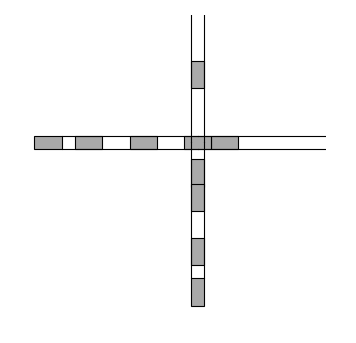
\includegraphics[width=0.38\textwidth]{../figures/single_intersection_example.png}
  \caption{Illustration of a single intersection with vehicles drawn as grey
    rectangles. Vehicles approach the intersection from the east and from the
    south and cross it without turning. Note that the first two waiting vehicles
    on the south lane kept some distance before the intersection, such that they
    are able to reach full speed whenever they
    cross.}\label{fig:single_intersection}
\end{figure}

\section*{Appendix A --- Preliminary results for single intersection}

\renewcommand{\thesection}{A}

This part presents the design of a neural scheduling heuristic for the offline
trajectory optimization problem with a single intersection. We discuss how these
results provide evidence that a similar methodology is feasible in a network of
intersections, thereby strengthening our belief that the proposed research
approach is set up to successfully answer research questions~\ref{Q1}
and~\ref{Q2}.
%
In this preliminary stage, we used an imitation learning setting to assess
whether the proposed model has enough capacity (``is complex enough'') to
capture policies that are close to optimal. In particular, we rely on expert
demonstration consisting of labeled transitions obtained from optimal solutions
computed by solving the equivalent MILP with Gurobi to train a certain
scheduling policy for generating solutions to the upper-level Vehicle Scheduling
Problem for a single intersection, which we show has a simple shape.

\subsection{Problem formulation}

Consider a single intersection with two incoming lanes, identified by indices
$\mathcal{R} = \{ 1, 2 \}$. The corresponding two routes are crossing the
intersection from south to north and crossing from west to east, see
Figure~\ref{fig:single_intersection}. We identify vehicles by their route and by
their relative order on this route, by defining the vehicle index set
\begin{align*}
  \mathcal{N} = \{ (r, k) : k \in \{1, \dots, n_{r}\}, r \in \mathcal{R}\} ,
\end{align*}
where $n_{r}$ denotes the number of vehicles following route $r$. Smaller values
of $k$ correspond to being closer to the intersection. Given vehicle index
$i = (r, k) \in \mathcal{N}$, we also use the notation $r(i) = r$ and $k(i) = k$.
%
We assume that each vehicle is represented by a rectangle of length $L$ and
width $W$ and that $x_{i}(t)$ is measured at the front bumper.
%
Consider the longitudinal dynamics of each vehicle $i$ along its route, for
which we use the well-known \textit{double integrator} model
\begin{align*}
  \dot{x}_{i}(t) = v_{i}(t) , \\
  \dot{v}_{i}(t) = u_{i}(t)  , \\
  0 \leq v_{i}(t) \leq v_{\max} , \\
  |u_{i}(t) | \leq a_{\max} ,
\end{align*}
where $x_{i}(t)$ is the vehicle's position, $v_{i}(t)$ its velocity and
$u_{i}(t)$ its acceleration, which is set by the central controller. Let
$D_{i}(s_{i,0})$ denote the set of all trajectories $x_{i}(t)$ satisfying these
dynamics, given some initial state $s_{i,0} = (x_{i}(0), v_{i}(0))$.
%
In order to
maintain a safe distance between consecutive vehicle on the same route, vehicle
trajectories need to satisfy
\begin{align*}
  x_{i}(t) - x_{j}(t) \geq L ,
\end{align*}
for all $t$ and all pairs of indices $i, j \in \mathcal{N}$ such that
$r(i) = r(j), k(i) + 1 = k(j)$. Let $\mathcal{C}$ denote the set of such ordered
pairs of indices, which we call \textit{conjunctive pairs}. Note that these
constraints restrict vehicle from overtaking each other, so the initial relative
order is maintained on each route.
%
For each $i \in \mathcal{N}$, let $\mathcal{E}_{i} = (B_{i}, E_{i})$ denote the
open interval such that vehicle $i$ occupies the intersection's conflict area if
and only if $B_{i} < x_{i}(t) < E_{i}$. Using this notation, collision avoidance
at the intersection is achieved by requiring
\begin{align*}
  (x_{i}(t), x_{j}(t)) \notin \mathcal{E}_{i} \times \mathcal{E}_{j} ,
\end{align*}
for all $t$ and for all pairs of indices $i, j \in \mathcal{N}$ with
$r(i) \neq r(j)$, which we collect in the set $\mathcal{D}$ and call \textit{disjunctive
  pairs}.
%
Suppose we have some performance criterion $J(x_{i})$ that takes into account
travel time and energy efficiency of the trajectory of vehicle $i$, then the
offline trajectory optimization problem for a single intersection can be
compactly written as
\begin{equation}
\label{eq:offline_single_intersection}
\begin{aligned}
  \min_{\mathbf{x}(t)} \quad & \sum_{i \in \mathcal{N}} J(x_{i}) \\
  \text{s.t.} \quad  & x_{i} \in D_{i}(s_{i,0}) , &\text{for all } i \in \mathcal{N} , \\
                & x_{i}(t) - x_{j}(t) \geq L, &\text{for all } (i,j) \in \mathcal{C} , \\
                & (x_{i}(t), x_{j}(t))  \notin \mathcal{E}_{i} \times \mathcal{E}_{j} , &\text{for all } \{i,j\} \in \mathcal{D} ,
\end{aligned}
\end{equation}
where $\mathbf{x}(t) = [\, x_{i}(t) : i \in \mathcal{N} \,]$ and all constraints
are meant to apply to all times $t$.


%\subsection{Direct transcription}
%
%Although computationally demanding,
%problem~\eqref{eq:offline_single_intersection} can be numerically solved by
%direct transcription to a mixed-integer linear program by
%discretization on a uniform time grid. Let $K$ denote the number of discrete
%time steps and let $\Delta t$ denote the time step size.
%%
%Using the forward Euler integration scheme, we have
%\begin{align*}
%  x_{i}(t + \Delta t) = x_{i}(t) + v_{i}(t) \Delta t , \\
%  v_{i}(t + \Delta t) = v_{i}(t) + u_{i}(t) \Delta t ,
%\end{align*}
%for each $t \in \{0, \Delta t, \dots, (K-1) \Delta t\}$. Following the approach
%in~\cite{hultApproximateSolutionOptimal2015}, the collision-avoidance
%constraints between routes can be formulated using the well-known big-M technique
%by the constraints
%\begin{align*}
%  x_{i}(t) \leq B_{i} + \delta_{i}(t) M , \\
%  E_{i} - \gamma_{i}(t) M \leq x_{i}(t) , \\
%  \delta_{i}(t) + \delta_{j}(t) + \gamma_{i}(t) + \gamma_{j}(t) \leq 3 ,
%\end{align*}
%where $\delta_{i}(t), \gamma_{i}(t) \in \{ 0, 1 \}$ for all $i \in \mathcal{N}$ and $M$ is a
%sufficiently large number.
%%
%Finally, the safe distance constraints can simply be added as
%\begin{align*}
%  x_{i}(t) - x_{j}(t) \geq L ,
%\end{align*}
%for each $t \in \{0, \Delta t, \dots, K \Delta t\}$ and each pair of consecutive
%vehicles $(i, j) \in \mathcal{C}$ on the same route.
%%
%For example, consider the objective functional
%\begin{align*}
%  J(x_{i}) = \int_{t=0}^{t_{f}} \left( {(v_{d} - v_{i}(t))}^{2} + {u_{i}(t)}^{2} \right) dt ,
%\end{align*}
%where $v_{d}$ is some reference velocity and $t_{f}$ denotes the final simulation time,
%then examples of optimal trajectories are shown in
%Figure~\ref{fig:direct_transcription_example}, corresponding to the initial conditions in Table~\ref{tab:hult_parameters}.
%
%\begin{table}[H]
%  \centering
%\caption{Example initial conditions $s_{i,0} = (x_{i}(0), v_{i}(0))$ for
%  problem~\eqref{eq:offline_single_intersection}.}\label{tab:hult_parameters}
%\vspace{0.5em}
%\begin{tabular}{ c | c c c | c c }
%  $i$  & (1,1) & (1,2) & (1,3) & (2,1) & (2,2) \\
%  \hline
%  $x_{i}(0)$ & 15 & 10 &  0 & 10 &  0 \\
%  $v_{i}(0)$ & 10 & 10 & 10 & 10 & 10 \\
%\end{tabular}
%\end{table}
%
%\begin{figure}[t]
%  \centering
%  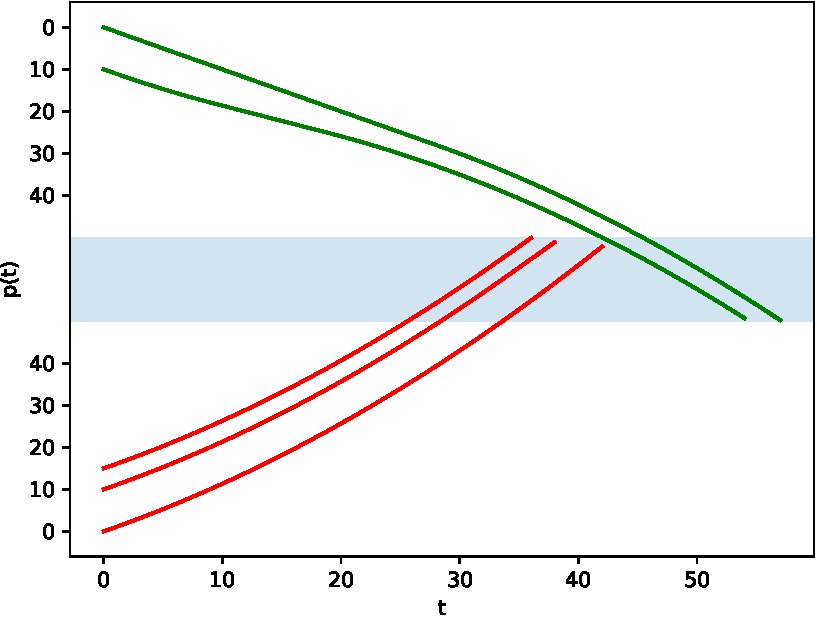
\includegraphics[width=0.7\textwidth]{../figures/direct_transcription_example.pdf}
%  \caption{Example of optimal trajectories obtained using the direct
%    transcription method with
%    $L = 5, \, \mathcal{E}_{i} \equiv \mathcal{E} = [50, 70], \, v_{d} = 20, \; T=120, \, \Delta t = 0.1$
%    and initial conditions as given in Table~\ref{tab:hult_parameters}. The
%    y-axis is split such that each part corresponds to one of the two routes and
%    the trajectories are inverted accordingly and drawn with separate colors.
%    The intersection area $\mathcal{E}$ is drawn as a shaded region. Whenever a
%    vehicle has left the intersection, we stop drawing its trajectory for
%    clarity.}
%  \label{fig:direct_transcription_example}
%\end{figure}


\subsection{Bilevel decomposition}

For the case where only a single vehicle is approaching the intersection for
each route, so $n_{r} = 1$ for all $r \in \mathcal{R}$, it has been shown
that problem~\eqref{eq:offline_single_intersection} can be decomposed into two coupled optimization problems, see
Theorem 1 in~\cite{hultApproximateSolutionOptimal2015}. Roughly speaking, the \textit{upper-level problem} optimizes the time
slots during which vehicles occupy the intersection, while the \textit{lower-level problems}
produce optimal safe trajectories that respect these time slots.
%
When allowing multiple vehicles per route, we show (without rigorous proof) that
a similar decomposition exists.
%
Given trajectory $x_{i}(t)$, the \textit{crossing time} of vehicle $i$ --- when the vehicle
first enters the intersection --- and the corresponding \textit{exit time} are, respectively,
\begin{align*}
  \inf \{ t: x_{i}(t) \in \mathcal{E}_{i} \}  \; \text{ and } \; \sup \{ t: x_{i}(t) \in \mathcal{E}_{i} \} .
\end{align*}
%
We will write $y(i)$ for the crossing time decision variable and write
$y(i) + \sigma(i)$ for the exit time. It turns out that trajectories can be generated
separately for each route, which yields a decomposition with upper-level problem
%
\begin{equation}
\begin{aligned}
  \min_{y, \sigma} \quad & \sum_{r \in \mathcal{R}} F(y_{r}, \sigma_{r}) \\
  \text{ s.t. } \quad & y(i) + \sigma(i) \leq y(j) \text{ or } y(j) + \sigma(j) \leq y(i), & \text{ for all } (i, j) \in \mathcal{D} , \\
  & (y_{r}, \sigma_{r}) \in \mathcal{S}_{r} , & \text{ for all } r \in \mathcal{R} ,
\end{aligned}
\end{equation}
where $F(y_{r}, \sigma_{r})$ and $\mathcal{S}_{r}$ are the value function and
set of feasible parameters, respectively, of the lower-level \textit{route trajectory optimization}
problems
\begin{equation}
\begin{aligned}
  F(y_{r}, \sigma_{r}) = \min_{x_{r}} \quad & \sum_{i \in \mathcal{N}(r)} J(x_{i}) \\
  \text{ s.t. } \quad & x_{i} \in D_{i}(s_{i,0}) , & \text{ for all } i \in \mathcal{N}_{r} , \\
  & x_{i}(y(i)) = B_{i} , & \text{ for all } i \in \mathcal{N}_{r} , \\
  & x_{i}(y(i) + \sigma(i)) = E_{i} , & \text{ for all } i \in \mathcal{N}_{r} , \\
  & x_{i}(t) - x_{j}(t) \geq L , & \text{ for all } (i, j) \in \mathcal{C} \cap \mathcal{N}_{r} ,
\end{aligned}
\end{equation}
where we use the notation $\mathcal{N}_{r} = \{ i \in \mathcal{N} : r(i) = r \}$ and
similarly for $x_{r}, y_{r}$ and $\sigma_{r}$ to group variables by route. Note that
the set of feasible parameters $\mathcal{S}_{r}$ implicitly depends on the
initial states $\{s_{i,0} : i \in \mathcal{N}_{r}\}$ and system parameters.

\subsubsection{Bilevel decomposition for delay objective}

In general, the upper- and lower-level problems are tightly coupled. However,
the problem becomes much easier when we assume that the trajectory performance
criterion is exactly the crossing time, so
$J(x_{i}) = \inf \{ t: x_{i}(t) \in \mathcal{E}_{i} \}$. In this case, we simply
have
\begin{align*}
  F(y_{r}, \sigma_{r}) \equiv F(y_{r}) = \sum_{i \in \mathcal{N}_{r}} y(i) .
\end{align*}
%
Furthermore, we assume that vehicles enter the network and cross the
intersection at full speed, so $v_{i}(0) = v_{i}(y(i)) = v_{\max}$, such that we
have
\begin{align*}
\sigma(i) \equiv \sigma = (L + W) / v_{\max}, \; \text{ for all } i \in \mathcal{N} ,
\end{align*}
see Figure~\ref{fig:vehicle_crossing}.
%
Therefore, we ignore the part related to $\sigma$ in the set of feasible parameters
$\mathcal{S}_{r}$, which can then be shown that to have a particularly simple
structure under these assumptions.
% earliest time of arrival
Observe that $r_{i} = (B_{i} - x_{i}(0)) / v_{\max}$ is the earliest time at
which vehicle $i$ can enter the intersection, when it keeps driving at maximum
velocity.
%
Let $\rho = L / v_{\max}$ be such that $y(i) + \rho$ is the time at which the rear
bumper of a crossing vehicle reaches the start line of the intersection, see
Figure~\ref{fig:vehicle_crossing}, then it can be shown that
$y_{r} \in \mathcal{S}_{r}$ if and only if
\begin{align*}
  r_{i} \leq y(i), \quad & \text{ for all } i \in \mathcal{N}_{r} , \\
  y(i) + \rho \leq y(j), \quad & \text{ for all } (i,j) \in \mathcal{C} \cap \mathcal{N}_{r} .
\end{align*}
Therefore, under the stated assumptions,
problem~\eqref{eq:offline_single_intersection} reduces to the following \textit{crossing time scheduling} problem
\begin{subequations}
  \label{eq:single_intersection_scheduling}
\begin{align}
  \min_{y} \quad & \sum_{i \in \mathcal{N}} y(i) \\
  \text{ s.t. } \quad & r_{i} \leq y(i) , & \text{ for all } i \in \mathcal{N} , \\
                    & y(i) + \rho \leq y(j) , & \text{ for all } (i,j) \in \mathcal{C} , \label{eq:conjunctions} \\
                    & y(i) + \sigma \leq y(j) \text{ or } y(j) + \sigma \leq y(i) , & \text{ for all } (i,j) \in \mathcal{D} \label{eq:disjunctions} ,
\end{align}
\end{subequations}
which can be solved using off-the-shelf mixed-integer linear program solvers,
after encoding the \textit{disjunctive constraints}~\eqref{eq:disjunctions} using the big-M
technique. Given optimal $y^{*}$, any set of trajectories
$[x_{i}(t) : i \in \mathcal{N}]$ that satisfies
\begin{align*}
  x_{i} \in D_{i}(s_{i,0}) , \quad & \text{ for all } i \in \mathcal{N} , \\
  x_{i}(y^{*}(i)) = B_{i} , \quad & \text{ for all } i \in \mathcal{N} , \\
  x_{i}(y^{*}(i) + \sigma) = E_{i} , \quad & \text{ for all } i \in \mathcal{N} , \\
  x_{i}(t) - x_{j}(t) \geq L , \quad & \text{ for all } (i,j) \in \mathcal{C} ,
\end{align*}
forms a valid solution. These trajectories can be computed by an efficient
direct transcription method. First, note that each route may be considered
separately. Trajectories on each route can then be computed in a sequential
manner by repeatedly solving the optimal control problem
%
\begin{align*}
\texttt{MotionSynthesize}(\tau, B, s_{0}, x') := \\
  {\arg\min}_{x: [0, \tau] \rightarrow \mathbb{R}} & \int_{0}^{\tau} |x(t)| dt \\
  \text{ s.t. } & \ddot{x}(t) = u(t) , &  \text{ for all } t \in [0, \tau] , \\
  & |u(t)| \leq a_{\max} , &  \text{ for all } t \in [0, \tau] , \\
  & 0 \leq \dot{x}(t) \leq v_{\max} , &  \text{ for all } t \in [0, \tau] , \\
  & x'(t) - x(t) \geq L , &  \text{ for all } t \in [0, \tau] , \\
  & (x(0), \dot{x}(0)) = s_{0} , \\
  & (x(\tau), \dot{x}(\tau)) = (B, v_{\max}) ,
\end{align*}
where $\tau$ is set to the required crossing time, $B$ denotes the distance to the
intersection, $s_{0}$ is the initial state of the vehicle and $x'$ denotes the
trajectory of the vehicle preceding the current vehicle, which is required to
maintain a safe following distance between the two vehicles.

\subsubsection{Extension to networks of intersections}

% similar bilevel decomposition under delay objective for network of intersections
% - upper level crossing time scheduling problem at intersections
% - lower level crossing time scheduling problem for each route
% - need to add additional constraints
% - buffer constraints
% - travel constraints

We briefly explain why we think that the above setup can be extended to a
network of intersections, thereby strengthening our belief that we can
successfully answer research question~\ref{Q1}.
%
First of all, the upper-level problem can be extended by considering a crossing
time variable $y(i, v)$ for every intersection $v$ on the route $r(i)$ of each
vehicle $i\in \mathcal{N}$. Given a valid schedule $y$ of crossing times, we can
then imagine a similar lower-level trajectory optimization problem that
generates collision-free trajectories for every vehicle. The main difficulty is
making sure that the constraints in the upper-level problem, which we denoted by
$(y_{r}, \sigma_{r}) \in \mathcal{S}_{r}$, are such that schedules $y$ always
result in a feasible lower-level problem.

We identify at least two new types of constraints that need to be considered in
a network. We need to take into account the time that vehicles need to drive
towards the next intersection on their route, which requires some kind of
\textit{travel constraints}, which can be defined relatively straightforward in
the current model. Furthermore, lanes between intersections can only provide
room for a finite number of driving or waiting vehicles, requiring some sort of
\textit{buffer constraints}. We expect that it is nontrivial to define these and
prove their correctness, since we need to take into account a combination of
both position and velocity of vehicles entering a lane.


\subsection{Crossing time scheduling}

Partial solutions to the crossing time scheduling
problem~\eqref{eq:single_intersection_scheduling} can be represented
clearly by their \textit{disjunctive graph}, which we define next. Let
$(\mathcal{N}, \mathcal{C}, \mathcal{O})$ be a directed graph with nodes
$\mathcal{N}$ and the following two types of arcs. The \textit{conjunctive arcs}
encode the fixed order of vehicles having the same route. For each
$(i,j) \in \mathcal{C}$, an arc from $i$ to $j$ means that vehicle $i$ reaches
the intersection before $j$ due to the follow
constraints~\eqref{eq:conjunctions}. The \textit{disjunctive arcs} are used to
encode the decisions regarding the ordering of vehicles on distinct routes,
corresponding to constraints~\eqref{eq:disjunctions}. For each pair
$\{i,j\} \in \mathcal{D}$, at most one of the arcs $(i,j)$ and $(j,i)$ can be
present in $\mathcal{O}$.

When $\mathcal{O} = \varnothing$, we say the disjunctive graph is
\textit{empty}. Each feasible schedule satisfies exactly one of the two
constraints in~\eqref{eq:disjunctions}. When $\mathcal{O}$ contains exactly one arc from every pair
of opposite disjunctive arcs, we say the disjunctive graph is \textit{complete}.
Note that such graph is acyclic and induces a unique topological ordering $\pi$
of its nodes. Conversely, every ordering $\pi$ of nodes $\mathcal{N}$ corresponds
to a unique complete disjunctive graph, which we denote by
$G(\pi) = (\mathcal{N}, \mathcal{C}, \mathcal{O}(\pi))$.

% edge weights
We define weights for every possible arc in a disjunctive graph. Every
conjunctive arc $(i, j) \in \mathcal{C}$ gets weight $w(i,j) = \rho_{i}$ and every
disjunctive arc $(i, j) \in \mathcal{O}$ gets weight $w(i,j) = \sigma_{i}$. Given
some vehicle ordering $\pi$, for every $j \in \mathcal{N}$, we recursively define
the lower bound
\begin{align}
  \text{LB}_\pi(j) = \max\{ r_{j}, \max_{i \in N^{-}_{\pi}(j)} \text{LB}_\pi(i) + w(i,j) \} ,
\end{align}
where $N^{-}_{\pi}(j)$ denotes the set of in-neighbors of node $j$ in $G(\pi)$.
Observe that this quantity is a lower bound on the crossing time, i.e., every
feasible schedule $y$ with ordering $\pi$ must satisfy $y_{i} \geq \text{LB}_\pi(i)$
for all $i \in \mathcal{N}$.


\subsubsection{Branch-and-bound solution}

Optimization problem~\eqref{eq:single_intersection_scheduling} can be turned into
a Mixed-Integer Linear Program (MILP) by rewriting the disjunctive constraints using
the well-known big-M method.
%
We introduce a binary decision variable $\gamma_{ij}$ for every
disjunctive pair $\{i, j\} \in \mathcal{D}$.
%
To avoid redundant variables, we first impose some arbitrary ordering of the
disjunctive pairs by defining
\begin{align*}
  \bar{\mathcal{D}} = \{ (i,j) : \{i,j\} \in \mathcal{D}, \; r(i) < r(j) \} ,
\end{align*}
such that for every $(i,j) \in \bar{\mathcal{D}}$, setting $\gamma_{ij} = 0$
corresponds with choosing disjunctive arc $i \rightarrow j$ and
$\gamma_{ij} = 1$ corresponds to $j \rightarrow i$. This yields the following
MILP formulation
%
\begin{align*}
  \min_{y} \quad & \sum_{i \in \mathcal{N}} y_{i} & \\
  \text{s.t.} \quad & r_{i} \leq y_{i}, & \text{ for all } i \in \mathcal{N} , \\
  & y_{i} + \rho_{i} \leq y_{j}, & \text{ for all } (i,j) \in \mathcal{C} , \label{eq:conjunctions} \\
  & y_{i} + \sigma_{i} \leq y_{j} + \gamma_{ij}M, & \text{ for all } (i,j) \in \bar{\mathcal{D}} , \\
  & y_{j} + \sigma_{j} \leq y_{i} + (1 - \gamma_{ij})M, & \text{ for all } (i,j) \in \bar{\mathcal{D}} , \\
  & \gamma_{ij} \in \{0, 1\}, & \text{ for all } (i,j) \in \bar{\mathcal{D}} ,
\end{align*}
where $M > 0$ is some sufficiently large number, which may depend on the
specific problem instance.


\subsubsection{Neural construction heuristic}

Define partial ordering $\pi$ to be a \textit{partial permutation} of
$\mathcal{N}$, which is a sequence of elements from some subset
$\mathcal{N}(\pi) \subset \mathcal{N}$.
%
Let $\pi$ be a partial ordering of length $n$ and let
$i \notin \mathcal{N}(\pi)$, then we use $\pi' = \pi \mdoubleplus i$ to denote
the concatenation of sequence $\pi$ with $i$, so $\pi'_{1:n} = \pi_{1:n}$ and
$\pi'_{n+1} = i$. Furthermore, recursively define the concatenation of two
sequences by
$\pi \mdoubleplus \pi' = ( \pi \mdoubleplus \pi'_{1} ) \mdoubleplus \pi'_{2:m}$,
where $m$ is the length of $\pi'$.
%
For each partial ordering $\pi$, the corresponding disjunctive graph $G(\pi)$ is
incomplete, meaning that some of the disjunctive arcs have not yet been added.
Nevertheless, observe that $\text{LB}_{\pi}(i)$ is still defined for every
$i \in \mathcal{N}$.
%
Let $\text{obj}(\pi)$ denote the objective of a complete ordering $\pi$.

% route ordering automaton
Observe that, due to the conjunctive constraints, ordering vehicles is
equivalent to ordering routes. We will define heuristics in terms of repeatedly
choosing to which route the next vehicle in the ordering belongs. It may be
helpful to model this as a deterministic finite-state automaton, where the set
of route indices $\mathcal{R}$ acts as the input alphabet. Let $S$ denote the
state space and let $\delta: S \times \mathcal{R} \rightarrow S$ denote the state-transition
function.

% states
Let $s$ denote an instance of~\eqref{eq:single_intersection_scheduling}. We
consider $s$ to be a fixed part of the state, so it does not change with state
transitions.
The other part of the state is the current partial ordering $\pi$.
% transitions
The transitions of the automaton are very simple. Let $(s, \pi) \in S$ denote
the current state and let $r \in \mathcal{R}$ denote the next symbol. Let
$i \in \mathcal{N} \setminus \mathcal{N}(\pi)$ denote the next unscheduled vehicle on route $r$,
then the system transitions to $(s, \pi \mdoubleplus i)$. If no such vehicle exists, the
transition is undefined.
%
% multi-step transition
% With a little abuse of notation, let $\delta(s, \eta) = \delta(s_{0}, \eta)$ denote the
% state that we obtain after applying sequence $\eta$ to the automaton with initial
% state $s_{0} = (s, \varnothing)$, which generalizes the single step transition function by
% recursively defining
% \begin{align*}
%   \delta(s_{0}, \eta_{1:t}) = \delta(\delta(s_{0}, \eta_{1:t-1}), \eta_{t}) .
% \end{align*}
%
Therefore, an input sequence $\eta$ of routes is called a \textit{valid route
  order} whenever it is of length
\begin{align*}
  N = \sum_{r \in \mathcal{R}} n_{r}
\end{align*}
and contains precisely $n_r$ occurrences of route $r \in \mathcal{R}$. Given
problem instance $s$, let $y_{\eta}(s)$ denote the schedule corresponding to route
order $\eta$. We say that route order $\eta$ is optimal whenever $y_{\eta}(s)$ is optimal.
Observe that an optimal route order must exist for every instance $s$, since we
can simply derive the route order from an optimal vehicle order.

Instead of mapping an instance $s$ directly to some optimal route order, we
consider a mapping $p : S \rightarrow \mathcal{R}$ such that setting $s_{0} = (s, \varnothing)$ and
repeatedly evaluating
\begin{align*}
  s_{t} = \delta(s_{t-1}, p(s_{t-1}))
\end{align*}
yields a final state $s_{N}(s, \pi^{*})$ with optimal schedule $\pi^{*}$.
Observe that this mapping must exist, because given some optimal route order
$\eta^{*}$, we can set $p(s_{t}) = \eta^{*}_{t+1}$, for every $t \in \{0, \dots, N-1\}$.

We do not hope to find an explicit representation of $p$, but our aim is to find
good heuristic approximations.
For example, consider the following simple \textit{threshold rule}.
%
Let $\pi$ denote a partial schedule of length $n$, so $i=\pi(n)$ is the last
scheduled vehicle with route $\texttt{last}(\pi)=r(i)$, then define
\begin{align*}
  p_{\tau}(s, \pi) = \begin{cases}
                \texttt{last}(\pi) \quad &\text{ if } \text{LB}_{\pi}(i) + \rho_{i} + \tau \geq r_{j} \text{ and } (i,j) \in \mathcal{C} , \\
                \texttt{next}(\pi) & \text{ otherwise, }
              \end{cases}
\end{align*}
for some threshold parameter $\tau \geq 0$. The expression $\texttt{next}(\pi)$ represents some
route other than $\texttt{last}(\pi)$ with unscheduled vehicles left.


\subsubsection{Imitation learning}

% We model the conditional distribution
% $p_{\theta}(\eta | s)$ of the optimal route sequence given a problem instance $s$
% and we factorize it as
% %
% \begin{align*}
%   p_{\theta} (\eta \, | \, s) = \prod_{t=1}^{N} p_{\theta}(\eta_{t} \, | \; \delta(s, \eta_{1:t-1})) ,
% \end{align*}
% %
% where $\theta$ denotes the model parameters.

Instead of explicitly formulating heuristics using elementary rules, we will now
consider a data-driven approach. To this end, we model the conditional
distribution $p_{\theta}(\eta_{t+1} | s_{t})$ with parameters $\theta$.
%
Consider an instance $s$ and some optimal route sequence $\eta$ with
corresponding states defined as $s_{t+1} = \delta(s_{t}, \eta_{t+1})$ for
$t \in \{0, \dots, N-1\}$. The resulting set of pairs $(s_{t}, \eta_{t+1})$ can be
used to learn $p_{\theta}$ in a supervised fashion by treating it as a classification
task.

% inference
Schedules are generated by employing \textit{greedy inference} as follows. The
model $p_{\theta}$ provides a distribution over routes. We ignore routes that have
no unscheduled vehicles left and take the argmax of the remaining probabilities.
We will denote the corresponding complete schedule by $\hat{y}_{\theta}(s)$.

Next, we discuss the parameterization of the model. We first derive, for every
$r \in \mathcal{R}$, a \textit{route embedding} $h(s_{t}, r)$ based on the current non-final state
$s_{t} = (s, \pi_{t})$ of the automaton.
%
Let $k_{\pi}(r)$ denote the first unscheduled vehicle in route $r$ under the partial schedule $\pi_{t}$.
Denote the smallest lower bound of unscheduled vehicles as
\begin{align*}
  T_{\pi} = \min_{i \in \mathcal{N} \setminus \mathcal{N}(\pi)} \text{LB}_{\pi}(i) .
\end{align*}
Let the \textit{horizon} of route $r$ be defined as
\begin{align*}
  h'(s_{t}, r) = ( \text{LB}_{\pi_{t}}(k_{\pi_{t}}(r)) - T_{\pi_{t}}, \dots, \text{LB}_{\pi_{t}}(n_{r}) - T_{\pi_{t}} ) .
\end{align*}
%
Observe that horizons can be of arbitrary dimension. Therefore, we restrict each
horizon to a fixed length $\Gamma$ and use zero padding. More precisely, given a
sequence $x = (x_{1}, \dots, x_{n})$ of length $n$, define the padding
operator
\begin{align*}
  \text{pad}(x, \Gamma) = \begin{cases}
                            (x_{1}, \dots, x_{\Gamma}), &\text{ if } \Gamma \leq n,  \\
                            (x_{1}, \dots, x_{n}) \mdoubleplus (\Gamma - n) * (0), &\text{ otherwise, }
                            \end{cases}
\end{align*}
where we use the notation $n * (0)$ to mean a sequence of $n$ zeros.
%
The route embedding is then defined as
\begin{align*}
  h(s_{t}, r) = \text{pad}(h'(s_{t}, r), \Gamma).
\end{align*}
%
Next, these are then arranged into a \textit{state embedding}
$h(s_{t})$ as follows. Let $\eta_{t}$ be the route that was chosen last, then we
apply the following \textit{route cycling} trick in order to keep the most recent route in
the same position of the state embedding, by defining
\begin{align*}
  h_{r}(s_{t}) = h(s_{t}, \; r - \eta_{t} \; \mathrm{mod} \; |\mathcal{R}|) ,
\end{align*}
for every $r \in \mathcal{R}$.
%
This state embedding is then mapped to a probability distribution
\begin{align*}
  p_{\theta}(\eta_{t+1} | s_{t}) = f_{\theta}(h(s_{t})) ,
\end{align*}
where $f_{\theta}$ is a fully connected neural network.

% \paragraph{Recurrent embedding.}
%
% To avoid the zero padding operation, which can be problematic for states that
% are almost done, we can employ a recurrent architecture that is agnostic to the
% number of remaining unscheduled vehicles. Each variable-length horizon
% $h'(s_{t}, l)$ is simply transformed into the fixed-length vector by an Elman
% RNN by taking the output at the last step.

% {\color{blue} Need to further specify
%   this, but the current implementation is working.}
% \begin{align*}
%   h(s_{t}, l) = \text{RNN}(h'(s_{t}, l)) .
% \end{align*}


\subsubsection{Experiments and discussion}

First, we define some classes of problem instances that we will use as a benchmark.
%
Instances are generated by sampling values of $g_{i} \sim G$ and $\rho_{i} \sim R$ according
to the parameters given in Table~\ref{tab:params} and setting
\begin{align*}
  r_{i} = \sum_{k=1}^{k(i)} g_{i} + \sum_{k=1}^{k(i) - 1} \rho_{i} ,
\end{align*}
for each $i \in \mathcal{N}$.
%
For each set specification in Table~\ref{tab:params}, we sample 1000 instances.

We solve each instance's MILP to optimality to obtain the training data set
$\mathcal{X}$, consisting of all the pairs $(s_{t}, \eta_{t+1})$ of state and next
route belonging to the optimal schedules.
% threshold heuristic fitting
We fit the simple threshold heuristic to $\mathcal{X}$ by finding the value of
$\tau$ with the lowest mean objective using a simple grid search.
%
% The fitted values are given in Table~\ref{tab:tau_opt}. Note that these values
% are all remarkably close, so we wonder if there is any dependency on $\rho_{i}$ or
% $\sigma$, because these are the only variables kept constant among the instance sets.
%
% neural heuristics fitting
In order to fit the model parameters of the neural models, we interpret
$p_{\theta}(s_{t})$ as the probability of choosing the first route and use the
binary cross entropy loss, defined as
\begin{align*}
  - \frac{1}{|\mathcal{X}|} \sum_{(s_{t}, \eta_{t+1}) \in \mathcal{X}} \mathds{1}\{\eta_{t+1} = 1\} \log(p_{\theta}(s_{t})) + \mathds{1}\{\eta_{t+1} = 2\} \log(1 - p_{\theta}(s_{t})) ,
\end{align*}
where $\mathds{1}(\cdot)$ denotes the indicator function.
%
We use 5 epochs with batch size 10 and we use learning rate $10^{-3}$ with the
Adam optimizer.

% evaluation
Let $\mathcal{Y}$ denote one of the test instance sets. Let $\text{obj}(y)$
denote the objective of schedule $y$, and let $\hat{y}$ denote the schedule
obtained from a heuristic, then Table~\ref{tab:objectives} reports on the
average approximation ratio defined as
\begin{align*}
  \alpha_{\text{approx}} = \frac{1}{|\mathcal{Y}|} \sum_{s \in \mathcal{Y}} \text{obj}(\hat{y}(s)) \; / \; \text{obj}(y^{*}(s))
\end{align*}
and the fraction of instances that are solved to optimality, which
we define as
\begin{align*}
  \alpha_{\text{opt}} = \frac{1}{|\mathcal{Y}|} \sum_{s \in \mathcal{Y}} \mathds{1}\{ \text{obj}(\hat{y}(s)) = \text{obj}(y^{*}(s)) \} .
\end{align*}


Observe that the policy parameterization is complex enough to model near-optimal
constructive policies for this single intersection scheduling problem. However,
these results should be interpreted with some care, as the very simple threshold
policy also achieves very close to optimal performance, which might suggest that
there is some fundamental structure hidden in the problem.
%
The fact that the relatively simple neural policy is able to capture the
apparent structure in the problem for a single intersection gives us hope to
obtain similar results whenever we consider a network of intersections. This
provides some motivation that research question~\ref{Q2} might eventually allow
a positive answer.

% - single intersection allows ordering vehicles one-by-one
% - apparently, there is some (simple) structure in the problem that our neural scheduler is able to
%   capture using imitation learning


\begin{table}[H]
  \caption{Specification of test instance sets. The total number of vehicles is
    shown as the sum of the number of vehicles per route $\sum n_{r}$. Every
    instance has switch-over time $\sigma = 2$.}\label{tab:params}
  \vspace{0.5em}
  \centering
  \begin{tabular}[t]{c c c c c c}
    \toprule
    set id & size & $|\mathcal{N}|$ & $G$ & $R$ \\
    \midrule

    1 & 100 & $10 + 10$ & $\text{Uni}(0, 4)$ & $1$ \\
    2 & 100 & $15 + 15$ & $\text{Uni}(0, 4)$ & $1$ \\
    3 & 100 & $20 + 20$ & $\text{Uni}(0, 4)$ & $1$ \\
    4 & 100 & $25 + 25$ & $\text{Uni}(0, 4)$ & $1$ \\ % too big for free Gurobi version

    5 & 100 & $10 + 10$ & $\text{Exp}(2)$    & $1$ \\
    6 & 100 & $15 + 15$ & $\text{Exp}(2)$    & $1$ \\

    \bottomrule
  \end{tabular}
\end{table}

% uses knitr to generate nice tables
%% silent package loading


\begin{knitrout}
\definecolor{shadecolor}{rgb}{0.969, 0.969, 0.969}\color{fgcolor}\begin{table}

\caption{\label{tab:unnamed-chunk-2}Solving times of Gurobi on the different sets of instances. Mean and standard deviation are given for the MILP without cutting planes (``plain''), type I cutting planes or both types of cutting planes. \label{tab:running_times}}
\centering
\begin{tabular}[t]{rlll}
\toprule
set id & plain & type I & type I + II\\
\midrule
1 & 0.084 $\pm$ 0.011 & 0.078 $\pm$ 0.004 & 0.087 $\pm$ 0.022\\
2 & 0.452 $\pm$ 0.007 & 0.314 $\pm$ 0.028 & 0.299 $\pm$ 0.134\\
3 & 2.525 $\pm$ 0.073 & 0.764 $\pm$ 0.267 & 0.837 $\pm$ 0.109\\
4 & 8.688 $\pm$ 5.326 & 2.486 $\pm$ 0.892 & 1.585 $\pm$ 0.045\\
\bottomrule
\end{tabular}
\end{table}

\end{knitrout}

%% silent package loading


\begin{knitrout}
\definecolor{shadecolor}{rgb}{0.969, 0.969, 0.969}\color{fgcolor}\begin{table}

\caption{\label{tab:unnamed-chunk-2}Approximation ratio for the heuristics. \label{tab:objectives}}
\centering
\begin{tabular}[t]{rr}
\toprule
set id & threshold $\tau = 1.2$\\
\midrule
1 & 1.026537\\
2 & 1.017220\\
3 & 1.011988\\
4 & 1.011209\\
6 & 1.026830\\
\addlinespace
7 & 1.026359\\
\bottomrule
\end{tabular}
\end{table}

\end{knitrout}

%% silent package loading


\begin{knitrout}
\definecolor{shadecolor}{rgb}{0.969, 0.969, 0.969}\color{fgcolor}\begin{table}[H]
\centering
\caption{\label{tab:unnamed-chunk-2}Optimal values of threshold parameter $\tau$ of the threshold
    heuristic, fitted using a simple grid search on each training data
    set.  \label{tab:tau_opt}}
\centering
\begin{tabular}[t]{ccccccc}
\toprule
set id & 1 & 2 & 3 & 4 & 5 & 6\\
\midrule
$\tau$ & 1.10 & 1.10 & 1.00 & 0.90 & 1.10 & 1.10\\
\bottomrule
\end{tabular}
\end{table}

\end{knitrout}


\begin{knitrout}
\definecolor{shadecolor}{rgb}{0.969, 0.969, 0.969}\color{fgcolor}\begin{table}[H]
\centering
\caption{\label{tab:unnamed-chunk-2}Mean approximation ratio
  $\alpha_\text{approx}$ and proportion of instances solved to optimality
  $\alpha_\text{opt}$. Evaluated for each set of test instances for the fitted
  \textit{threshold} heuristic and the fitted neural heuristic with
  \textit{padded} embedding. Each set contains 100
  instances. \label{tab:objectives}}
\vspace{0.5em}
\centering
\begin{tabular}[t]{rrrrr}
\toprule
\multicolumn{1}{c}{ } & \multicolumn{2}{c}{$\alpha_\text{approx}$} & \multicolumn{2}{c}{$\alpha_\text{opt}$} \\
\cmidrule(l{3pt}r{3pt}){2-3} \cmidrule(l{3pt}r{3pt}){4-5}
set id & threshold & padded &  threshold & padded \\
\midrule
1 & 1.0198 & 1.0085  & 0.12 & 0.33\\
2 & 1.0132 & 1.0102  & 0.12 & 0.20\\
3 & 1.0102 & 1.0079  & 0.11 & 0.17\\
4 & 1.0088 & 1.0054  & 0.05 & 0.13\\
5 & 1.0359 & 1.0120  & 0.19 & 0.35\\
6 & 1.0258 & 1.0110  & 0.12 & 0.23\\
\bottomrule
\end{tabular}
\end{table}

\end{knitrout}

\newpage

\section*{Appendix B --- In-depth discussion of related literature}

\renewcommand{\thesection}{B}
\setcounter{subsection}{0}

% There are numerous social and technological aspects to the design of traffic
% coordination systems.

\subsection{Traffic coordination}

A good example of an early centralized approach is the ``Autonomous Intersection
Management'' (AIM) paper~\cite{dresnerMultiagentApproachAutonomous2008}, which
is based on a reservation scheme. The conflict zone is modeled by a grid of
cells. Vehicles that want to cross the intersection send a request to the
central controller to occupy the cells containing its trajectory for a certain
amount of time. The central controller then decides to grant or deny these
requests based on previous granted requests, in order to facilitate
collision-free trajectories. If a request is denied, the vehicle slows down and
attempts to obtain a new reservation after some timeout.

% direct transcription
Optimal control problems can be approached in an end-to-end fashion by
\textit{direct transcription} to an equivalent mixed-integer optimization
problem, which can be solved using off-the-shelf solvers (e.g.,
SCIP~\cite{BolusaniEtal2024OO} or Gurobi~\cite{gurobi}). Such methods can be
used to compute optimal trajectories up to any precision, by choosing a fine
enough time discretization. However, it is exactly this time discretization that
causes prohibitive growth of the number of variables with respect to the size of
the network and the number of vehicles, so this method is only really useful for
toy problems.
%
Therefore, approximation schemes have been studied in previous
works~\cite{hultApproximateSolutionOptimal2015,zhaoBilevelProgrammingModel2021,tallapragadaHierarchicaldistributedOptimizedCoordination2017}.


% Hult et al. (offline single intersection with energy objective)
% "An approximate solution to the optimal coordination problem for autonomous
% vehicles at intersections"
The approximation method in~\cite{hultApproximateSolutionOptimal2015} is based
on this bilevel decomposition and considers an quadratic objective involving
velocity as a proxy for energy. The first stage optimizes a schedule of vehicle
crossing times. It uses approximations of each vehicle's contribution to the
total objective, as a function of its crossing time. Next, for each vehicle, the
second stage computes an optimal trajectory that satisfies the crossing time
schedule by solving a quadratic program. This approach has been shown to reduce
running times significantly. Unfortunately, this study is limited to a single
intersection and it is assumed that each lane approaching the intersection
contains exactly one vehicle.
% Zhao et al. (bilevel programming model)
The paper~\cite{zhaoBilevelProgrammingModel2021} proposes a trajectory
optimization scheme for a single intersection, also based on the bilevel
decomposition. The lower-level problem is employed to maximize the speed at
which vehicles enter the intersection. Both levels are solved in an alternating
fashion, each time updating the constraints of the other problem based on the
current solution.
% bubbles paper
The optimization scheme
in~\cite{tallapragadaHierarchicaldistributedOptimizedCoordination2017} deals
explicitly with the complexity of the crossing order decisions by defining
groups of consecutive vehicles on the same lane. The first step is to group
vehicles into these so-called ``bubbles''. All vehicles in a bubble are required
to cross the intersection together, while maintaining feasibility with respect
to safe trajectories. Next, crossing times are assigned to bubbles while
avoiding collisions. Based on this schedule, a local vehicular control
method~\cite{tallapragadaDistributedControlVehicle2017} is used that guarantees
safety to reach the assigned crossing times.

% \subsection{Job-shop scheduling}


% The buffer constraints we propose to add to the JSSP formulation are similar in
% nature to the constraints used in JSSP with limited buffer capacities,
% see~\cite{heitmannJobshopSchedulingLimited2007} for an introduction and
% heuristic solutions for this variant.

% Shifting bottleneck heuristic.

\subsection{Neural combinatorial optimization}

% maybe discuss traditional epsilon-approximation schemes?
% argue that it takes a lot of expert knowledge about the problem structure to design these

This section introduces the idea of applying a Machine Learning (ML) perspective
on Combinatorial Optimization (CO) problems, which has recently gained a lot of
attention. One of the key ideas in this line of research is to treat problem
instances as data points and to use machine learning methods to approximately
map them to corresponding optimal solutions~\cite{bengioMachineLearningCombinatorial2020}.
% learning assumptions:
% supervised learning (expert labels) vs reinforcement learning (experience)
It is very natural to see the sequential decision-making process of any
optimization algorithm in terms of the Markov Decision Process (MDP) framework,
where the environment corresponds to the internal state of the algorithm. From
this perspective, two main learning regimes can be distinguished.
% imitiation learning
Methods like those based on the branch-and-bound framework are
often computationally too expensive for practical purposes, so \textit{learning
  to imitate} the decisions taken in these exact algorithms might provide us
with fast approximations. In this approach, the ML model's performance is
measured in terms of how similar the produced decisions are to the
demonstrations provided by the expert.
% reinforcement learning
On the other hand, some problems do not even enable exact methods, so it is
interesting to study solution methods that \textit{learn from experience}. An
interesting feature of this kind of approach is that it enables us to implicitly
exploit the hidden structure of the problems we want to solve.

% neural combinatorial optimization
Because neural networks are commonly used as encoder in these ML models for CO,
we will refer to this new field as \textit{Neural Combinatorial Optimization} (NCO).
%
A wide range of classical combinatorial optimization problems has already been
considered in this framework, so we briefly discuss the taxonomy used in the
survey~\cite{mazyavkinaReinforcementLearningCombinatorial2020}.
% principal vs. joint approach
One distinguishing feature is whether existing off-the-shelf solvers are used or
not. On the one hand, \textit{principal} methods are based on a parameterized algorithm
that is tuned to directly map instances to solutions, while \textit{joint} methods
integrate with existing off-the-shelf solvers in some way (see the
survey~\cite{lodiLearningBranchingSurvey2017} on integration with the
branch-and-bound framework). An illustrative example of the latter category are
the use of ML models for the branching heuristic or the selection of cutting
planes in branch-and-cut algorithms~\cite{tangReinforcementLearningInteger2020}.
% principal - construction vs. improvement (guided search)
The class of principal methods can be further divided into \textit{construction}
heuristics, which produce complete solutions by repeatedly extending partial
solutions, and \textit{improvement} heuristics, which aim at iteratively improving the
current solution with some tunable search procedure.


% learning algorithms:
% REINFOCE with baseline
% Fitting the neural mapping is often done using policy gradient methods (with
% baseline), e.g., with the classical REINFORCE algorithm.

% constraints in differentiable models

A major challenge in NCO is constraint
satisfaction. For example, solutions produced by constructive neural policies
need to satisfy the constraints of the original combinatorial problem.
Therefore, an important question is how to enforce these constraints. To this
end, neural network architectures have been designed whose outputs satisfy some
kind of constraint, for example being a permutation of the
input~\cite{vinyalsPointerNetworks2017a}. Constraints can also be enforced by
the factorization of the mapping into repeated application of some policy. For
example, in methods for TSP, a policy is defined that repeatedly selects the
next node to visit. The constraint that nodes may be only visited once can be
easily enforced by ignoring the visited nodes and taking the argmax among the
model's probabilities for unvisited nodes.


% encoders:
% standard multilayer perceptron networks are not suited to encode order
% pointer networks
% graph neural networks


% examples for job-shop scheduling
Various NCO methods have already been studied for JSSP with makespan objective,
of which we now highlight some works that illustrate some of the above classes
of methods. A lot of the policies used in these works rely on some graph neural
network architecture, which is why the survey~\cite{smitGraphNeuralNetworks2024}
provides an overview based on this distinguishing feature.

% Tassel (principal construction, naive environment)
A very natural approach to model JSSP in terms of an MDP is taken
in~\cite{tasselReinforcementLearningEnvironment2021}, where a dispatching
heuristic is defined in an environment based on discrete scheduling time steps.
%
Every available job corresponds to a valid action and there is a so-called No-Op
action to skip to the next time step. States are encoded by some manually
designed features. They consider the makespan objective by proposing a dense
reward based on how much idle time is introduced compared to the processing time
of the job that is dispatched.
%
In some situation, some action can be proved to be always optimal (``non-final
prioritization''), in which case the policy is forced to take this action.
Additionally, the authors design some rules for when the No-Op action is not
allowed in order to prevent unnecessary idling of machines.
%
The proposed method is evaluated on the widely used
Taillard~\cite{taillardBenchmarksBasicScheduling1993} and
Demirkol~\cite{DEMIRKOL1998137} benchmarks, for which performance is compared to
static dispatching rules and a constraint programming (CP) solver, which is
considered cutting-edge.

% exact start times follow from order
From a scheduling theory
perspective~\cite{pinedoSchedulingTheoryAlgorithms2016}, it can be shown that
optimal schedules are completely characterized by the order of operations for
regular objectives (non-decreasing functions of the completion times). The start
times are computed from this order by a so-called \textit{placement rule}, so
considering discrete time steps introduces unnecessary model redundancy.

% Zhang construction heuristic (principal construction, based on order)

The seminal ``Learning to Dispatch'' (L2D)
paper~\cite{zhangLearningDispatchJob2020} proposes a construction heuristic for
JSSP with makespan objective. Their method is based on a dispatching policy that
is parameterized in terms of a graph neural network encoding of the disjunctive
graph belonging to a partial solution. Again, each action corresponds to
choosing for which job the next operation is dispatched. The rewards are based
on how much the lower bound on the makespan changes between consecutive states.
They use a Graph Isomorphism Network (GIN) architecture to parameterize both an
actor and critic, which are trained using the Proximal Policy Optimization (PPO)
algorithm. Using the Taillard and Demirkol benchmarks, they show that their
model is able to generalize well to larger instances.
% problem with dispatching mechanism
As we already alluded to above, this way of modeling the environment is better
suited to JSSP with regular objectives, because it does not explicitly determine
starting times.
%
They use a dispatching mechanism based on finding the earliest starting time of
a job, even before already scheduled jobs, see their Figure 2. By doing this,
they introduce symmetry in the environment: after operations
$O_{11}, O_{21}, O_{31}$ have been scheduled, both action sequences
$O_{22}, O_{32}$ and $O_{32}, O_{22}$ lead to exactly the same state $S_5$ shown
in their Figure 2. In this particular example, this means that it is impossible
to have $O_{11} \rightarrow O_{22} \rightarrow O_{32}$. In general, it is not
clear whether the resulting restricted policy is still sufficiently powerful, in
the sense that an optimal operation order can always be constructed.

% Zhang improvement heuristic (principal improvement)

Recently, the authors of L2D investigated an improvement heuristic for
JSSP~\cite{zhangDeepReinforcementLearning2024} with makespan objective.
%
This method is based on selecting a solution within the well-known $N_5$
neighborhood, which has been used in previous local search heuristics.
%
It is still not clear whether their resulting policy is complete, in the sense
that any operation order can be achieved by a sequence of neighborhood moves.
%
The reward is defined in terms of how much the solution improves relative to the
best solution seen so far (the ``incumbent'' solution). The policy is
parameterized using a GIN architecture designed to capture the topological
ordering of operations encoded in the disjunctive graph of solutions. They
propose a custom $n$-step variant of the REINFORCE algorithm in order to deal
with the sparse reward signal and long trajectories.
%
To compute the starting times based on the operation order, they propose a
dynamic programming algorithm, in terms of a message-passing scheme, as a more
efficient alternative to the classical recursive critical path method.
%
Our proposal for efficiently updating the current starting time lower bounds in
partial solutions can also be understood as a similar message-passing scheme,
but where only some messages are necessary.

% Tassel (joint with CP solver)
An example of a joint method is given in~\cite{tasselEndEndReinforcementLearning2023}, where the environment is stated in
terms of a Constraint Programming (CP) formulation. This allows the method to be
trained using demonstration from an off-the-shelf CP solver.

% backpropagation through solution
Instead of enforcing constraints by developing some tailored model architecture,
like constructive and improvement heuristics, general methodologies have
recently been explored for the problem of constraint satisfaction in neural
networks. For example, the DC3 framework~\cite{dontiDC3LearningMethod2021}
employs two differentiable processes, completion and correction, to solve any
violations of equality or inequality constraints, respectively. The more recent
HardNet framework~\cite{minHardConstrainedNeuralNetworks2024} uses a closed-form
projection to map to feasible solutions under affine constraints and relies on a
differentiable convex optimization solver (e.g.,
OptNet~\cite{amosOptNetDifferentiableOptimization2021}) when general convex
constraints are considered.

\end{document}
